% The GPU-Native Persistent Actor Model
% Technical Paper - arXiv Preprint Style
%
% Describes a paradigm for treating GPU compute units as actors with
% persistent kernels, lock-free message passing, and causal ordering.
%
% Implementations: RingKernel (Rust), DotCompute (.NET), Orleans.GpuBridge, RustGraph
%
% Target: arXiv (cs.DC, cs.PL, cs.AR)
%
\documentclass[11pt,letterpaper]{article}

%% ============================================================================
%% arXiv-style formatting
%% ============================================================================

% Page geometry - generous margins for readability
\usepackage[
    letterpaper,
    top=1in,
    bottom=1in,
    left=1.25in,
    right=1.25in
]{geometry}

% Typography
\usepackage[T1]{fontenc}
\usepackage{lmodern}              % Latin Modern fonts
\usepackage{microtype}            % Improved typography
\usepackage{setspace}
\setstretch{1.15}                 % Slightly increased line spacing

% Math
\usepackage{amsmath}
\usepackage{amssymb}
\usepackage{amsthm}

% Tables and figures
\usepackage{booktabs}
\usepackage{multirow}
\usepackage{subcaption}
\usepackage{graphicx}
\usepackage{float}

% Code listings
\usepackage{listings}
\usepackage{xcolor}

% Graphics
\usepackage{tikz}
\usepackage{pgfplots}
\pgfplotsset{compat=1.16}
\usetikzlibrary{shapes,arrows,positioning,fit,calc}

% References and links
\usepackage{hyperref}
\usepackage{url}
\usepackage[numbers,sort&compress]{natbib}

% Author handling
\usepackage{authblk}
\usepackage{orcidlink}            % ORCID icons

%% ============================================================================
%% Hyperref setup
%% ============================================================================
\hypersetup{
    colorlinks=true,
    linkcolor=blue!70!black,
    filecolor=magenta,
    urlcolor=blue!70!black,
    citecolor=green!50!black,
    pdftitle={The GPU-Native Persistent Actor Model},
    pdfauthor={Michael Ivertowski},
    pdfsubject={GPU Computing, Actor Model, Distributed Systems},
    pdfkeywords={Actor Model, GPU, CUDA, Persistent Kernels, HLC}
}

%% ============================================================================
%% Code listing styles
%% ============================================================================

% Rust
\lstdefinelanguage{Rust}{
  keywords={fn, let, mut, if, else, match, for, while, loop, return, struct, enum, impl, trait, pub, use, mod, async, await, self, Self, where, type, const, static, unsafe, extern, crate, super},
  keywordstyle=\color{blue!80!black}\bfseries,
  keywords=[2]{i32, i64, u32, u64, f32, f64, bool, usize, isize, String, Vec, Option, Result, Arc, Box, AtomicU32, AtomicU64},
  keywordstyle=[2]\color{teal!80!black},
  comment=[l]{//},
  morecomment=[s]{/*}{*/},
  commentstyle=\color{gray}\itshape,
  stringstyle=\color{red!70!black},
  morestring=[b]",
  basicstyle=\ttfamily\small,
  breaklines=true,
  showstringspaces=false,
  tabsize=2,
}

% CUDA
\lstdefinelanguage{CUDA}{
  language=C++,
  morekeywords={__global__, __device__, __shared__, __host__, threadIdx, blockIdx, blockDim, gridDim, atomicAdd, atomicCAS, __syncthreads, __threadfence},
  keywordstyle=\color{blue!80!black}\bfseries,
  commentstyle=\color{gray}\itshape,
  stringstyle=\color{red!70!black},
  basicstyle=\ttfamily\small,
  breaklines=true,
  showstringspaces=false,
}

\lstset{
  language=Rust,
  frame=single,
  framerule=0.5pt,
  rulecolor=\color{gray!50},
  numbers=left,
  numberstyle=\tiny\color{gray},
  xleftmargin=2em,
  framexleftmargin=1.5em,
  backgroundcolor=\color{gray!5},
  captionpos=b,
}

%% ============================================================================
%% Custom commands
%% ============================================================================
\newcommand{\arxiv}[1]{\href{https://arxiv.org/abs/#1}{arXiv:#1}}
\newcommand{\github}[1]{\href{https://github.com/#1}{\texttt{github.com/#1}}}

%% ============================================================================
%% Document metadata
%% ============================================================================

\title{%
    \LARGE\textbf{The GPU-Native Persistent Actor Model:}\\[0.3em]
    \Large\textbf{Bringing Actor Semantics to Massively Parallel Hardware}
}

\author[1]{Michael Ivertowski~\orcidlink{0009-0008-7829-2249}}
\affil[1]{%
    Ernst \& Young AG\\
    Zurich, Switzerland\\
    \texttt{michael.ivertowski@ch.ey.com}
}

\date{%
    January 2026\\[1em]
    \small\textit{Preprint. Under review.}
}

%% ============================================================================
%% Document
%% ============================================================================
\begin{document}

\maketitle

%% Abstract
\begin{abstract}
\noindent
% Abstract
% Target: 150-250 words summarizing the key contributions

The actor model, introduced by Hewitt in 1973, has become foundational for building
concurrent and distributed systems. However, existing implementations target CPU
architectures, leaving GPU parallelism largely unexplored for actor-based computation.
We present the \textbf{GPU-Native Persistent Actor Model}, a paradigm that treats GPU
compute units as long-running actors with lock-free message passing and causal ordering.

This paper describes \textbf{RingKernel}, the Rust implementation of this paradigm,
alongside three companion frameworks: \textbf{DotCompute} (.NET), \textbf{Orleans.GpuBridge}
(Microsoft Orleans integration), and \textbf{RustGraph} (living graph database). Together,
these systems demonstrate the broad applicability of GPU-native actors.

Our key contributions are: (1) formalization of GPU actor semantics with Host-to-Kernel (H2K),
Kernel-to-Host (K2H), and Kernel-to-Kernel (K2K) messaging channels; (2) a 128-byte
\texttt{ControlBlock} structure for GPU-resident actor lifecycle management; (3) integration
of Hybrid Logical Clocks (HLC) for causal ordering across thousands of concurrent GPU actors;
and (4) cross-language implementations proving the paradigm's universality.

We evaluate on NVIDIA RTX Ada GPUs, demonstrating that persistent GPU actors achieve
\textbf{11,327$\times$ lower latency} for interactive commands compared to traditional
kernel launches (0.03$\mu$s vs 317$\mu$s). For mixed workloads, GPU-native actors achieve
\textbf{2.7$\times$ higher throughput}. RustGraph's P0-P4 GPU optimizations deliver
\textbf{3.51$\times$ fused kernel speedup}, \textbf{68\% work-stealing success rate},
and \textbf{124.7 million edges/second} peak throughput. Compared to sequential CPU execution,
the GPU living graph achieves \textbf{2--12$\times$ speedup} for iterative algorithms
(crossover at $\sim$1,000 nodes) and \textbf{O(1) query latency} (3--17 ns vs O(n) recomputation).
The unified hypergraph demo showcases \textbf{20 analytics across 6 categories}---GPU living,
behavioral, temporal, audit (ISA 240/315/570, SOX 404), compliance (AML/KYC), and accounting---spanning
64+ algorithms in 15 domains. This enables real-time fraud detection, enterprise compliance
monitoring, and distributed digital twins.

\end{abstract}

\vspace{1em}
\noindent\textbf{Keywords:} Actor Model, GPU Computing, Persistent Kernels, Message Passing, Hybrid Logical Clocks, Lock-Free Algorithms, CUDA, WebGPU, Distributed Systems, Graph Analytics

\vspace{0.5em}
\noindent\textbf{ACM CCS:} Computer systems organization $\rightarrow$ Parallel architectures; Software and its engineering $\rightarrow$ Concurrent programming structures

\vspace{1.5em}

%% Main content sections
% Section 1: Introduction

\section{Introduction}
\label{sec:introduction}

The actor model, proposed by Hewitt, Bishop, and Steiger in 1973~\cite{hewitt1973actors},
provides a powerful abstraction for concurrent computation. An actor is a computational
entity that, in response to a message, can: (1) send messages to other actors, (2) create
new actors, and (3) modify its own private state. This model has proven remarkably
successful for building fault-tolerant distributed systems, with implementations like
Erlang~\cite{armstrong2003erlang}, Akka~\cite{akka2023}, and Microsoft
Orleans~\cite{bykov2011orleans} powering critical infrastructure at companies like
WhatsApp, Twitter, and Microsoft.

However, the actor model has remained largely confined to CPU architectures. Modern GPUs
offer massive parallelism---thousands of cores executing concurrently---yet GPU
programming models like CUDA and OpenCL treat the GPU as a \emph{batch processor} rather
than an \emph{interactive system}. The conventional pattern is to launch a kernel,
wait for completion, and repeat. This ``launch-per-operation'' model incurs significant
overhead for interactive workloads.

\subsection{The Kernel Launch Problem}

Traditional GPU programming follows a strict pattern:
\begin{enumerate}
    \item Allocate device memory
    \item Copy input data from host to device
    \item Launch kernel
    \item Synchronize (wait for completion)
    \item Copy results from device to host
    \item Deallocate memory
\end{enumerate}

Each kernel launch involves driver overhead, PCIe transfers, and synchronization costs.
For a single operation, this overhead is negligible compared to computation time.
However, for \emph{interactive workloads}---where the host frequently sends commands
to an ongoing GPU computation---the overhead dominates. Our measurements show kernel
launch overhead of approximately 317$\mu$s on modern NVIDIA GPUs, making interactive
command rates above 3,000 commands/second impractical.

\subsection{Persistent Kernels: A Partial Solution}

The persistent kernel pattern~\cite{gupta2012persistent,steinberger2014whippletree}
addresses launch overhead by keeping a kernel running indefinitely. Instead of launching
per operation, a single kernel runs continuously and polls for work. Research has shown
speedups of up to 211$\times$ for workloads requiring many kernel invocations~\cite{wu2015persistent}.

However, existing persistent kernel work focuses on \emph{performance optimization},
not \emph{programming model}. The semantics remain imperative: the kernel is a loop
that checks flags and processes data. There is no abstraction for actors, messages,
supervision, or fault tolerance.

\subsection{Our Contribution: GPU-Native Actors}

We present \textbf{RingKernel}, a system that applies actor model semantics to GPU
computing. Our key insight is that GPU threads (or thread blocks) can be viewed as
actors: they have private state (registers, shared memory), communicate via messages
(through lock-free queues), and run persistently.

RingKernel makes the following contributions:

\begin{enumerate}
    \item \textbf{Formalization of GPU Actor Semantics} (\S\ref{sec:design}): We extend
    the actor model with three communication channels---Host-to-Kernel (H2K),
    Kernel-to-Host (K2H), and Kernel-to-Kernel (K2K)---that map naturally to GPU
    memory hierarchies.

    \item \textbf{ControlBlock Architecture} (\S\ref{sec:implementation}): We introduce
    a 128-byte GPU-resident structure that manages actor lifecycle, including activation,
    heartbeat, and graceful termination.

    \item \textbf{Hybrid Logical Clocks on GPU} (\S\ref{sec:implementation}): We implement
    HLC~\cite{kulkarni2014hlc} for causal ordering of messages across GPU actors,
    enabling distributed systems semantics on massively parallel hardware.

    \item \textbf{Rust-to-CUDA Transpilation} (\S\ref{sec:implementation}): We provide
    a DSL and transpiler that generates persistent kernel CUDA code from high-level
    Rust actor definitions, including automatic message envelope handling.

    \item \textbf{Comprehensive Evaluation} (\S\ref{sec:evaluation}): We demonstrate
    11,327$\times$ lower command latency and 2.7$\times$ higher mixed-workload
    throughput compared to traditional GPU programming on NVIDIA RTX Ada.
\end{enumerate}

\subsection{Paper Organization}

The remainder of this paper is organized as follows. Section~\ref{sec:background}
provides background on the actor model and GPU programming. Section~\ref{sec:related}
discusses related work. Section~\ref{sec:design} presents the RingKernel system design.
Section~\ref{sec:implementation} details the implementation. Section~\ref{sec:evaluation}
evaluates performance. Section~\ref{sec:discussion} discusses limitations and future
work. Section~\ref{sec:conclusion} concludes.

% Section 2: Background

\section{Background}
\label{sec:background}

This section provides background on the actor model and GPU programming,
establishing the concepts that RingKernel unifies.

\subsection{The Actor Model}

The actor model~\cite{hewitt1973actors} is a mathematical model of concurrent computation.
An \emph{actor} is an autonomous computational agent with three capabilities:

\begin{enumerate}
    \item \textbf{Send messages} to actors whose addresses (``acquaintances'') it knows
    \item \textbf{Create new actors} with specified behavior
    \item \textbf{Designate behavior} for handling the next message received
\end{enumerate}

Critically, actors \emph{cannot} share state---they interact only through asynchronous
message passing. This restriction eliminates data races by construction, making reasoning
about concurrent systems tractable.

\subsubsection{Actor Semantics}

Actors process messages from a \emph{mailbox} (message queue) one at a time. Message
delivery is guaranteed but \emph{unordered}---if actor $A$ sends messages $m_1$ and $m_2$
to actor $B$, they may arrive in any order. However, within a single actor, message
processing is sequential.

The operational semantics can be expressed as a transition relation:
\begin{equation}
    \langle \mathcal{A}, \mathcal{M} \rangle \rightarrow \langle \mathcal{A}', \mathcal{M}' \rangle
\end{equation}
where $\mathcal{A}$ is the set of actors, $\mathcal{M}$ is the multiset of in-flight
messages, and the transition represents processing one message.

\subsubsection{Supervision and Fault Tolerance}

Erlang introduced the concept of \emph{supervision}~\cite{armstrong2003erlang}: actors
are organized into hierarchies where parent actors monitor children. When a child fails,
the supervisor can restart it, escalate the failure, or take other recovery actions.
This ``let it crash'' philosophy enables building fault-tolerant systems.

\subsubsection{Causal Ordering}

In distributed actor systems, establishing message ordering is essential for consistency.
\emph{Lamport timestamps}~\cite{lamport1978clocks} provide partial ordering based on
causality: if event $a$ ``happens before'' event $b$ (written $a \rightarrow b$), then
$C(a) < C(b)$ where $C$ is the clock function.

\emph{Hybrid Logical Clocks} (HLC)~\cite{kulkarni2014hlc} combine physical time with
logical counters:
\begin{equation}
    \text{HLC} = \langle \text{physical\_time}, \text{logical\_counter}, \text{node\_id} \rangle
\end{equation}
HLC provides the causal ordering guarantees of Lamport clocks while maintaining
proximity to wall-clock time.

\subsection{GPU Architecture and Programming}

Modern GPUs contain thousands of cores organized hierarchically. We focus on NVIDIA
CUDA architecture, though the concepts generalize.

\subsubsection{Execution Model}

CUDA organizes computation into a hierarchy:
\begin{itemize}
    \item \textbf{Thread}: Smallest execution unit, has private registers
    \item \textbf{Warp}: 32 threads executing in SIMT lockstep
    \item \textbf{Block}: Collection of warps sharing fast ``shared memory''
    \item \textbf{Grid}: Collection of blocks executing the same kernel
\end{itemize}

\subsubsection{Memory Hierarchy}

GPU memory is organized by access speed and scope:
\begin{itemize}
    \item \textbf{Registers}: Per-thread, fastest (1 cycle latency)
    \item \textbf{Shared Memory}: Per-block, fast (5-10 cycles)
    \item \textbf{L1/L2 Cache}: Automatic caching of global memory
    \item \textbf{Global Memory}: Device-wide, slow (200-400 cycles)
    \item \textbf{Mapped Memory}: Host-visible, accessible from both CPU and GPU
\end{itemize}

Mapped memory is crucial for persistent kernels---it enables the host to communicate
with a running kernel without explicit memory copies.

\subsubsection{Synchronization Primitives}

CUDA provides several synchronization mechanisms:
\begin{itemize}
    \item \texttt{\_\_syncthreads()}: Block-level barrier
    \item \texttt{atomicAdd/CAS}: Atomic operations on global memory
    \item \textbf{Cooperative Groups} (CC 6.0+): Grid-level synchronization via
    \texttt{grid.sync()}
\end{itemize}

Cooperative groups enable persistent kernels to synchronize across all blocks, essential
for iterative algorithms like stencil computations.

\subsubsection{Traditional Kernel Launch Model}

The conventional CUDA programming pattern treats kernels as \emph{batch operations}:

\begin{lstlisting}[language=CUDA, caption={Traditional kernel launch pattern}]
// Host code
float *d_input, *d_output;
cudaMalloc(&d_input, size);
cudaMalloc(&d_output, size);
cudaMemcpy(d_input, h_input, size, H2D);

process_kernel<<<grid, block>>>(d_input, d_output);
cudaDeviceSynchronize();  // Block until complete

cudaMemcpy(h_output, d_output, size, D2H);
cudaFree(d_input);
cudaFree(d_output);
\end{lstlisting}

Each kernel launch involves driver API calls, command buffer submission, and
synchronization overhead---typically 10-500$\mu$s depending on GPU and driver.

\subsection{Mapping Actors to GPUs}

Table~\ref{tab:actor-gpu-mapping} shows how actor model concepts map to GPU primitives:

\begin{table}[h]
\centering
\caption{Mapping between Actor Model and GPU concepts}
\label{tab:actor-gpu-mapping}
\begin{tabular}{@{}ll@{}}
\toprule
\textbf{Actor Concept} & \textbf{GPU Equivalent} \\
\midrule
Actor & Persistent thread block \\
Private state & Shared memory + registers \\
Mailbox & Lock-free ring buffer in global memory \\
Message send & Atomic enqueue operation \\
Message receive & Atomic dequeue operation \\
Actor creation & Dynamic parallelism (limited) \\
Supervision & Host thread monitoring ControlBlock \\
\bottomrule
\end{tabular}
\end{table}

This mapping forms the foundation of RingKernel's design.

% Section 3: Related Work

\section{Related Work}
\label{sec:related}

The GPU-native actor model builds upon decades of research in actor systems, GPU computing,
and persistent kernel techniques. We survey related work and position our contributions.

\subsection{Actor Model Implementations}

\subsubsection{Erlang and the BEAM VM}

Erlang~\cite{armstrong2003erlang} pioneered practical actor systems with its lightweight
processes, fault-tolerant supervision trees, and ``let it crash'' philosophy. The BEAM
virtual machine supports millions of concurrent processes with preemptive scheduling and
soft real-time garbage collection. Elixir~\cite{elixir2023} provides modern syntax atop BEAM.

While Erlang excels at CPU-bound concurrent workloads, it has no native GPU support.
GPU operations require NIFs (Native Implemented Functions) that break Erlang's
scheduling guarantees.

\subsubsection{Akka and the JVM}

Akka~\cite{akka2023} brings actor semantics to the JVM, supporting both classic and
typed actors. Akka Cluster enables distributed actors across machines with location
transparency. Akka Streams provides backpressure-aware message processing.

Like Erlang, Akka targets CPU architectures. While JNI can invoke CUDA, this creates
the same semantic mismatch as Erlang NIFs.

\subsubsection{Microsoft Orleans}

Orleans~\cite{bykov2011orleans} introduces ``virtual actors'' that are automatically
instantiated on demand and garbage collected when idle. This simplifies distributed
programming by hiding actor lifecycle management. Orleans powers backend services at
Microsoft, including Xbox Live and Azure.

Orleans' virtual actor model is compelling for cloud services but assumes network
communication costs dominate---the opposite of GPU's memory hierarchy.

\subsubsection{Other Implementations}

Pony~\cite{clebsch2015pony} provides actors with reference capabilities for data-race
freedom. CAF (C++ Actor Framework)~\cite{caf2023} offers native performance.
Ray~\cite{moritz2018ray} targets distributed machine learning with actor-like ``tasks.''
None provide GPU-native actors.

\subsection{Persistent Kernel Techniques}

\subsubsection{Persistent Threads}

Gupta et al.~\cite{gupta2012persistent} formalized persistent threads (PT) as a GPU
programming technique where threads run indefinitely, polling for work. They demonstrated
up to 211$\times$ speedup for fine-grained workloads by eliminating kernel launch overhead.

Steinberger et al.~\cite{steinberger2014whippletree} extended PT with dynamic task
scheduling, enabling irregular workloads on GPUs. Their Whippletree system achieves
high utilization for variable-length tasks.

\subsubsection{PERKS}

Huangfu et al.~\cite{huangfu2022perks} introduced PERKS (PERsistent KernelS) for
iterative memory-bound applications. By moving the time loop inside the kernel and
using device-wide barriers, PERKS achieves 2.29$\times$ speedup for stencil computations
on NVIDIA A100.

PERKS focuses on performance for structured iterative patterns. The GPU-native actor
model extends this with actor semantics---message passing, lifecycle management, and
causal ordering---for general concurrent applications.

\subsubsection{GPU-Initiated Communication}

Agostini et al.~\cite{agostini2017gpu} demonstrated GPU-initiated communication using
GPUDirect RDMA and NVSHMEM. Their work enables GPU threads to directly send network
messages without host intervention.

K2K messaging applies similar principles at the device level, enabling direct
kernel-to-kernel communication through mapped memory.

\subsection{Lock-Free Data Structures on GPU}

\subsubsection{GPU Queue Implementations}

Cederman and Tsigas~\cite{cederman2008queue} implemented lock-free queues on GPUs
using atomic compare-and-swap (CAS). Their work demonstrated that lock-free algorithms
can achieve high throughput on GPU architectures.

Tzeng et al.~\cite{tzeng2010task} developed task queues for GPU ray tracing, handling
dynamic work distribution without locks. Their approach influenced GPU work-stealing
designs.

The GPU-native actor model uses single-producer single-consumer (SPSC) ring buffers
with atomic head/tail pointers, optimized for the H2K/K2H communication pattern.

\subsubsection{Memory Consistency}

Alglave et al.~\cite{alglave2015gpu} formalized GPU memory consistency models,
identifying subtle differences from CPU models. Their work is essential for
correct lock-free programming on GPUs.

Our implementations use memory fences ({\tt \_\_threadfence()}) and atomic operations
following NVIDIA's relaxed memory model guidelines.

\subsection{Causal Ordering in Distributed Systems}

\subsubsection{Logical Clocks}

Lamport's logical clocks~\cite{lamport1978clocks} provide partial ordering based on
causality. Vector clocks~\cite{fidge1988timestamps,mattern1989virtual} capture full
causality but have $O(n)$ space complexity.

\subsubsection{Hybrid Logical Clocks}

Kulkarni et al.~\cite{kulkarni2014hlc} introduced Hybrid Logical Clocks (HLC) that
combine physical time with logical counters. HLC provides causality guarantees while
staying close to wall-clock time, with $O(1)$ space per timestamp.

All GPU-native actor implementations use HLC for causal ordering across thousands
of concurrent GPU actors---a novel contribution enabling distributed systems semantics
on massively parallel hardware.

\subsection{GPU Programming Languages and DSLs}

\subsubsection{High-Level GPU Languages}

Futhark~\cite{henriksen2017futhark} provides a functional data-parallel language
that compiles to CUDA/OpenCL. Halide~\cite{ragan2013halide} separates algorithms from
schedules for image processing. Neither targets persistent actor patterns.

\subsubsection{Rust GPU Ecosystems}

rust-gpu~\cite{rustgpu2023} compiles Rust to SPIR-V for Vulkan/WebGPU compute shaders.
cudarc~\cite{cudarc2023} provides safe Rust bindings to CUDA driver/runtime APIs.
RingKernel builds on cudarc for runtime management and provides its own Rust-to-CUDA
transpiler for actor kernel generation.

\subsection{GPU-Native Actor Ecosystem}

Beyond RingKernel, three companion frameworks implement the GPU-native actor paradigm,
demonstrating its applicability across languages and domains.

\subsubsection{DotCompute (.NET 9/C\#)}

DotCompute is a universal compute acceleration framework for .NET 9+ that implements
the Ring Kernel System for persistent GPU actors. Key features include:

\begin{itemize}
    \item \textbf{Multi-backend support}: CUDA, OpenCL, Metal, with CPU fallback
    \item \textbf{Message Queue Bridge}: Named host-side queues with background DMA
    transfer to GPU-resident ring buffers, achieving $\sim$1.24$\mu$s serialization
    \item \textbf{LINQ-to-GPU}: Automatic kernel generation from LINQ queries with
    kernel fusion optimization (50-80\% bandwidth reduction)
    \item \textbf{Native AOT}: Sub-10ms startup with full trimming support
    \item \textbf{Source generators}: Compile-time kernel generation via Roslyn
\end{itemize}

DotCompute achieves 21-92$\times$ speedup on CUDA compared to CPU baselines, with
a production deployment of 215/234 tests passing (91.9\%).

\subsubsection{Orleans.GpuBridge (.NET/Orleans)}

Orleans.GpuBridge integrates GPU-native actors with Microsoft Orleans' virtual actor
model, enabling distributed GPU computing across Orleans clusters:

\begin{itemize}
    \item \textbf{RingKernelGrainBase}: Orleans grains backed by persistent GPU kernels,
    achieving 100-500ns message latency vs 10-100$\mu$s for CPU actors
    \item \textbf{Hypergraph actors}: Multi-way relationships with GPU-accelerated
    pattern matching using CSR memory layout
    \item \textbf{Temporal causality}: HLC and vector clocks maintained on GPU
    \item \textbf{P2P GPU messaging}: NVLink/PCIe direct communication with automatic
    fallback to CPU-routed paths
    \item \textbf{Placement strategies}: Queue-depth-aware grain placement for
    GPU device affinity
\end{itemize}

Orleans.GpuBridge enables ``Knowledge Organisms''---emergent intelligence from
GPU actor interactions---with 2M messages/second per actor throughput.

\subsubsection{RustGraph (Rust)}

RustGraph implements a ``living graph database'' where nodes and edges are persistent
GPU actors that continuously maintain analytics state:

\begin{itemize}
    \item \textbf{GpuNodeState}: 256-byte actor state (2 cache lines) with inline
    analytics fields (PageRank, BFS distance, component ID, fraud scores)
    \item \textbf{K2K Ring Buffer Inboxes}: Per-node lock-free message queues
    (512 capacity default) with 100-500ns latency
    \item \textbf{64+ living analytics}: PageRank, eigenvector centrality,
    community detection, triangle counting---all maintained via message propagation
    \item \textbf{O(1) queries}: Analytics always current; queries read node state
    rather than computing on-demand
    \item \textbf{Audit analytics}: Three-way match, segregation of duties,
    fraud triangle scoring computed via actor message passing
    \item \textbf{Unified hypergraph}: Accounting, internal controls, and
    process mining domains in single GPU structure
\end{itemize}

RustGraph demonstrates that the GPU-native actor paradigm fundamentally changes
graph analytics from ``compute on demand'' to ``continuously maintained state.''

\subsection{Comparison Summary}

Table~\ref{tab:related-comparison} summarizes how the GPU-native actor ecosystem
relates to prior work:

\begin{table*}[t]
\centering
\caption{Comparison with related systems}
\label{tab:related-comparison}
\begin{tabular}{@{}lcccccc@{}}
\toprule
\textbf{System} & \textbf{Actor Semantics} & \textbf{GPU Native} & \textbf{Persistent} & \textbf{HLC} & \textbf{K2K} & \textbf{Language} \\
\midrule
Erlang/OTP & \checkmark & -- & -- & -- & \checkmark & Erlang \\
Akka & \checkmark & -- & -- & -- & \checkmark & Scala/Java \\
Orleans & \checkmark & -- & -- & -- & \checkmark & C\# \\
PERKS & -- & \checkmark & \checkmark & -- & -- & CUDA \\
Whippletree & -- & \checkmark & \checkmark & -- & -- & CUDA \\
NVSHMEM & -- & \checkmark & -- & -- & \checkmark & CUDA \\
\midrule
\textbf{RingKernel} & \checkmark & \checkmark & \checkmark & \checkmark & \checkmark & Rust \\
\textbf{DotCompute} & \checkmark & \checkmark & \checkmark & \checkmark & \checkmark & C\# \\
\textbf{Orleans.GpuBridge} & \checkmark & \checkmark & \checkmark & \checkmark & \checkmark & C\# \\
\textbf{RustGraph} & \checkmark & \checkmark & \checkmark & \checkmark & \checkmark & Rust \\
\bottomrule
\end{tabular}
\end{table*}

The GPU-native actor ecosystem is unique in combining actor model semantics with
GPU-native persistent execution, causal ordering via HLC, and direct kernel-to-kernel
communication. The four implementations share a common architecture while targeting
different domains: general GPU computing (RingKernel), .NET acceleration (DotCompute),
distributed virtual actors (Orleans.GpuBridge), and graph analytics (RustGraph).

Table~\ref{tab:ecosystem-comparison} compares the ecosystem implementations:

\begin{table*}[t]
\centering
\caption{GPU-Native Actor Ecosystem Comparison}
\label{tab:ecosystem-comparison}
\begin{tabularx}{\textwidth}{@{}l>{\raggedright\arraybackslash}X>{\raggedright\arraybackslash}X>{\raggedright\arraybackslash}X>{\raggedright\arraybackslash}X@{}}
\toprule
\textbf{Feature} & \textbf{RingKernel} & \textbf{DotCompute} & \textbf{Orleans.GpuBridge} & \textbf{RustGraph} \\
\midrule
Language & Rust & C\# (.NET 9) & C\# (Orleans) & Rust \\
GPU Backends & CUDA, WebGPU & CUDA, OpenCL, Metal & CUDA, DotCompute & CUDA \\
Primary Domain & FDTD simulation & General compute & Distributed actors & Graph analytics \\
Message Latency & 0.03\,$\mu$s & 1.24\,$\mu$s & 100--500\,ns & 100--500\,ns \\
Actor Granularity & Thread block & Thread block & Grain (virtual) & Graph node \\
Unique Feature & Rust-to-CUDA DSL & LINQ-to-GPU & Hypergraph actors & 64+ living analytics \\
Test Coverage & 900+ tests & 215/234 tests & 1,231 tests & 1,400+ tests \\
\bottomrule
\end{tabularx}
\end{table*}

% Section 4: System Design

\section{System Design}
\label{sec:design}

This section presents RingKernel's architecture, formalizing how actor model concepts
map to GPU execution.

\subsection{Design Goals}

RingKernel targets the following design goals:

\begin{enumerate}
    \item \textbf{Actor Semantics}: Provide message passing, private state, and
    lifecycle management matching traditional actor systems.

    \item \textbf{GPU Efficiency}: Minimize host-device communication and maximize
    GPU occupancy through persistent execution.

    \item \textbf{Causal Ordering}: Enable distributed systems reasoning with
    Hybrid Logical Clocks across GPU actors.

    \item \textbf{Zero-Copy Communication}: Use memory-mapped buffers to avoid
    explicit data transfers for control messages.

    \item \textbf{Ergonomic API}: Provide a Rust DSL that compiles to efficient
    CUDA while hiding low-level details.
\end{enumerate}

\subsection{System Architecture}

Figure~\ref{fig:architecture} shows RingKernel's high-level architecture.

\begin{figure}[h]
\centering
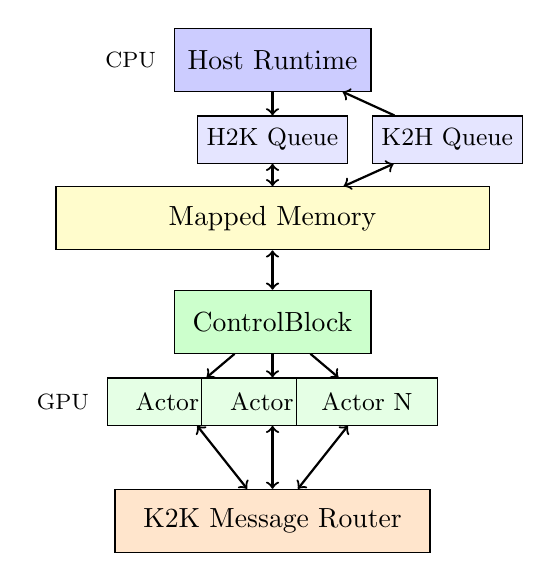
\begin{tikzpicture}[
    node distance=0.8cm,
    box/.style={rectangle, draw, minimum width=2.5cm, minimum height=0.8cm, align=center},
    smallbox/.style={rectangle, draw, minimum width=1.8cm, minimum height=0.6cm, align=center, font=\small},
    arrow/.style={->, thick}
]
    % Host side
    \node[box, fill=blue!20] (host) {Host Runtime};
    \node[smallbox, below=0.3cm of host, fill=blue!10] (h2k) {H2K Queue};
    \node[smallbox, right=0.3cm of h2k, fill=blue!10] (k2h) {K2H Queue};

    % Mapped memory region
    \node[box, below=1.2cm of host, fill=yellow!20, minimum width=5.5cm] (mapped) {Mapped Memory};

    % Device side
    \node[box, below=0.5cm of mapped, fill=green!20] (ctrl) {ControlBlock};
    \node[smallbox, below=0.3cm of ctrl, xshift=-1.2cm, fill=green!10] (actor1) {Actor 0};
    \node[smallbox, below=0.3cm of ctrl, fill=green!10] (actor2) {Actor 1};
    \node[smallbox, below=0.3cm of ctrl, xshift=1.2cm, fill=green!10] (actor3) {Actor N};

    % K2K messaging
    \node[box, below=0.8cm of actor2, fill=orange!20, minimum width=4cm] (k2k) {K2K Message Router};

    % Arrows
    \draw[arrow] (host) -- (h2k);
    \draw[arrow] (k2h) -- (host);
    \draw[arrow, <->] (h2k) -- (mapped);
    \draw[arrow, <->] (k2h) -- (mapped);
    \draw[arrow, <->] (mapped) -- (ctrl);
    \draw[arrow] (ctrl) -- (actor1);
    \draw[arrow] (ctrl) -- (actor2);
    \draw[arrow] (ctrl) -- (actor3);
    \draw[arrow, <->] (actor1) -- (k2k);
    \draw[arrow, <->] (actor2) -- (k2k);
    \draw[arrow, <->] (actor3) -- (k2k);

    % Labels
    \node[left=0.1cm of host, font=\footnotesize] {CPU};
    \node[left=0.1cm of actor1, font=\footnotesize] {GPU};
\end{tikzpicture}
\caption{RingKernel architecture showing Host-to-Kernel (H2K), Kernel-to-Host (K2H),
and Kernel-to-Kernel (K2K) communication through mapped memory.}
\label{fig:architecture}
\end{figure}

\subsection{Actor Model Extension for GPU}

We extend the traditional actor model with three distinct communication channels:

\subsubsection{Host-to-Kernel (H2K) Channel}

The H2K channel carries commands from the host application to GPU actors:
\begin{itemize}
    \item \texttt{RunSteps(n)}: Execute $n$ computation steps
    \item \texttt{InjectImpulse(pos, value)}: Inject data at position
    \item \texttt{Terminate}: Graceful shutdown request
    \item \texttt{GetProgress}: Query current state
\end{itemize}

H2K is implemented as an SPSC (Single-Producer Single-Consumer) ring buffer in
mapped memory. The host is the sole producer; thread block 0 on the GPU is the consumer.

\subsubsection{Kernel-to-Host (K2H) Channel}

The K2H channel carries responses from GPU actors to the host:
\begin{itemize}
    \item \texttt{Ack(cmd\_id)}: Command acknowledgment
    \item \texttt{Progress(step, energy)}: Progress report
    \item \texttt{Error(code, msg)}: Error notification
    \item \texttt{Terminated}: Shutdown confirmation
\end{itemize}

K2H is also an SPSC ring buffer with the GPU as producer and host as consumer.

\subsubsection{Kernel-to-Kernel (K2K) Channel}

The K2K channel enables direct communication between GPU actors without host intervention.
This is essential for algorithms requiring inter-block communication, such as:
\begin{itemize}
    \item Stencil halo exchange between spatial tiles
    \item Scatter-gather operations in graph algorithms
    \item Work stealing in dynamic load balancing
\end{itemize}

K2K uses device memory (not mapped) for minimal latency. A routing table maps
actor IDs to buffer addresses.

\subsection{GPU Actor Lifecycle}

GPU actors follow a defined lifecycle managed through the ControlBlock:

\begin{enumerate}
    \item \textbf{Initializing}: Actor is being set up (shared memory, state)
    \item \textbf{Active}: Actor is processing messages
    \item \textbf{Draining}: Actor is completing pending work before shutdown
    \item \textbf{Terminated}: Actor has stopped; resources can be reclaimed
\end{enumerate}

State transitions are atomic to prevent races:

\begin{lstlisting}[language=CUDA, caption={Atomic lifecycle transition}]
__device__ bool transition_to_active(ControlBlock* cb) {
    uint32_t expected = STATE_INITIALIZING;
    return atomicCAS(&cb->state, expected, STATE_ACTIVE)
           == expected;
}
\end{lstlisting}

\subsection{Message Envelope Format}

All messages use a standardized 256-byte envelope format:

\begin{lstlisting}[language=Rust, caption={Message envelope structure}]
#[repr(C, align(64))]
struct MessageHeader {
    magic: u64,           // 0x52494E474B45524E ("RINGKERN")
    version: u32,
    message_type: u32,
    payload_size: u32,
    flags: u32,
    source_kernel: u32,
    dest_kernel: u32,
    correlation_id: u64,
    hlc_physical: u64,    // HLC timestamp
    hlc_logical: u32,
    hlc_node_id: u32,
    checksum: u32,
    _reserved: [u8; 180], // Pad to 256 bytes
}
\end{lstlisting}

The 64-byte alignment ensures coalesced memory access. The magic number enables
validation of message integrity.

\subsection{Hybrid Logical Clocks on GPU}

RingKernel implements HLC for causal ordering. Each actor maintains an HLC:

\begin{lstlisting}[language=CUDA, caption={HLC operations on GPU}]
struct HlcClock {
    uint64_t physical;  // Wall clock (from host)
    uint32_t logical;   // Logical counter
    uint32_t node_id;   // Actor identifier
};

__device__ void hlc_send(HlcClock* clock, MessageHeader* msg) {
    uint64_t now = get_system_time();  // From ControlBlock
    if (now > clock->physical) {
        clock->physical = now;
        clock->logical = 0;
    } else {
        clock->logical++;
    }
    msg->hlc_physical = clock->physical;
    msg->hlc_logical = clock->logical;
    msg->hlc_node_id = clock->node_id;
}

__device__ void hlc_receive(HlcClock* clock, MessageHeader* msg) {
    uint64_t now = get_system_time();
    uint64_t msg_pt = msg->hlc_physical;
    if (now > clock->physical && now > msg_pt) {
        clock->physical = now;
        clock->logical = 0;
    } else if (clock->physical > now && clock->physical > msg_pt) {
        clock->logical++;
    } else if (msg_pt > now && msg_pt > clock->physical) {
        clock->physical = msg_pt;
        clock->logical = msg->hlc_logical + 1;
    } else {  // msg_pt == clock->physical
        clock->logical = max(clock->logical, msg->hlc_logical) + 1;
    }
}
\end{lstlisting}

This enables causal ordering across GPU actors: if actor $A$ sends message $m$ to
actor $B$, and $B$ sends message $m'$ after receiving $m$, then $m \rightarrow m'$
in the happens-before relation, reflected in HLC timestamps.

\subsection{Lock-Free Ring Buffer}

The message queues use lock-free SPSC ring buffers:

\begin{lstlisting}[language=CUDA, caption={Lock-free ring buffer}]
struct RingBuffer {
    volatile uint32_t head;  // Producer writes here
    volatile uint32_t tail;  // Consumer reads here
    uint32_t capacity;       // Power of 2
    uint32_t mask;           // capacity - 1
    uint8_t* data;           // Message storage
};

__device__ bool enqueue(RingBuffer* rb, void* msg, uint32_t size) {
    uint32_t head = rb->head;
    uint32_t next = (head + 1) & rb->mask;
    if (next == rb->tail) return false;  // Full

    memcpy(&rb->data[head * MSG_SIZE], msg, size);
    __threadfence();  // Ensure data visible before head update
    rb->head = next;
    return true;
}

__device__ bool dequeue(RingBuffer* rb, void* msg, uint32_t size) {
    uint32_t tail = rb->tail;
    if (tail == rb->head) return false;  // Empty

    memcpy(msg, &rb->data[tail * MSG_SIZE], size);
    __threadfence();  // Ensure read complete before tail update
    rb->tail = (tail + 1) & rb->mask;
    return true;
}
\end{lstlisting}

The power-of-2 capacity enables fast modulo via bitwise AND. Memory fences ensure
visibility across CPU-GPU boundary for mapped memory.

\subsection{ControlBlock Structure}

The 128-byte ControlBlock provides GPU-resident lifecycle management:

\begin{lstlisting}[language=Rust, caption={ControlBlock structure}]
#[repr(C, align(128))]
struct ControlBlock {
    // Lifecycle (8 bytes)
    state: AtomicU32,           // Lifecycle state
    flags: AtomicU32,           // Feature flags

    // Timing (24 bytes)
    heartbeat: AtomicU64,       // Last activity timestamp
    system_time: AtomicU64,     // Host-updated wall clock
    step_counter: AtomicU64,    // Computation steps completed

    // Configuration (16 bytes)
    kernel_id: u32,
    block_count: u32,
    queue_capacity: u32,
    _pad1: u32,

    // Statistics (32 bytes)
    messages_processed: AtomicU64,
    messages_sent: AtomicU64,
    errors: AtomicU64,
    _pad2: u64,

    // Reserved (48 bytes)
    _reserved: [u8; 48],
}
\end{lstlisting}

The host periodically updates \texttt{system\_time} and reads \texttt{heartbeat}
to detect stalled actors (watchdog pattern).

\subsection{Supervision Model}

RingKernel maps Erlang-style supervision to the host-GPU relationship:

\begin{itemize}
    \item \textbf{Host as Supervisor}: The host runtime monitors ControlBlock health,
    can terminate and restart GPU actors.

    \item \textbf{Actors as Children}: GPU thread blocks are supervised actors
    that can fail independently.

    \item \textbf{Recovery Strategies}:
    \begin{itemize}
        \item \texttt{Restart}: Relaunch kernel with fresh state
        \item \texttt{Resume}: Update ControlBlock to resume execution
        \item \texttt{Escalate}: Report failure to application
    \end{itemize}
\end{itemize}

The watchdog detects stalls by comparing \texttt{heartbeat} against
\texttt{system\_time}---if the difference exceeds a threshold, the actor is
considered failed.

% Section 5: Implementation

\section{Implementation}
\label{sec:implementation}

RingKernel is implemented in Rust with approximately 25,000 lines of code across
multiple crates. This section details key implementation aspects.

\subsection{Crate Architecture}

RingKernel is organized as a Cargo workspace:

\begin{itemize}
    \item \texttt{ringkernel-core}: Core traits, types, and enterprise features (457 tests)
    \item \texttt{ringkernel-derive}: Procedural macros for actor definitions
    \item \texttt{ringkernel-cpu}: CPU backend for testing and fallback
    \item \texttt{ringkernel-cuda}: NVIDIA CUDA backend with cudarc bindings
    \item \texttt{ringkernel-cuda-codegen}: Rust-to-CUDA transpiler (190+ tests)
    \item \texttt{ringkernel-wgpu}: WebGPU cross-platform backend
    \item \texttt{ringkernel-wgpu-codegen}: Rust-to-WGSL transpiler
    \item \texttt{ringkernel}: Facade crate re-exporting all functionality
\end{itemize}

\subsection{Rust-to-CUDA Transpilation}

The transpiler converts Rust DSL to CUDA C, enabling developers to write GPU
kernels in familiar syntax while generating optimized device code.

\subsubsection{Input: Rust Actor Definition}

\begin{lstlisting}[language=Rust, caption={Rust actor definition}]
#[ring_kernel(id = "processor", block_size = 128)]
fn handle(ctx: &RingContext, msg: &Request) -> Response {
    let tid = ctx.global_thread_id();

    // Shared memory reduction
    let partial = shared_reduce(msg.values, ReductionOp::Sum);

    ctx.sync_threads();

    if tid == 0 {
        Response { sum: partial, count: msg.values.len() }
    }
}
\end{lstlisting}

\subsubsection{Output: CUDA Kernel}

The transpiler generates a persistent kernel with message handling:

\begin{lstlisting}[language=CUDA, caption={Generated CUDA kernel (simplified)}]
extern "C" __global__ void processor_kernel(
    ControlBlock* cb,
    RingBuffer* h2k_queue,
    RingBuffer* k2h_queue,
    K2KRouter* k2k_router
) {
    __shared__ uint8_t shared_mem[4096];

    // Initialize HLC
    HlcClock hlc = {0, 0, cb->kernel_id};

    // Persistent message loop
    while (true) {
        // Check termination
        if (cb->state == STATE_TERMINATED) break;

        // Try receive from H2K
        MessageHeader header;
        if (try_dequeue(h2k_queue, &header)) {
            hlc_receive(&hlc, &header);

            switch (header.message_type) {
            case MSG_REQUEST:
                Request* req = (Request*)(h2k_queue->data
                    + header.payload_offset);
                Response resp = handle_request(req);

                // Send response
                MessageHeader resp_hdr;
                resp_hdr.correlation_id = header.correlation_id;
                hlc_send(&hlc, &resp_hdr);
                enqueue(k2h_queue, &resp_hdr, &resp);
                break;

            case MSG_TERMINATE:
                cb->state = STATE_TERMINATED;
                break;
            }
        }

        // Update heartbeat
        if (threadIdx.x == 0) {
            atomicExch(&cb->heartbeat, cb->system_time);
        }
    }
}
\end{lstlisting}

\subsubsection{Transpilation Pipeline}

The transpiler operates in phases:

\begin{enumerate}
    \item \textbf{Parse}: Convert Rust source to AST using \texttt{syn}
    \item \textbf{Analyze}: Extract types, identify GPU intrinsics, validate semantics
    \item \textbf{Transform}: Convert Rust constructs to CUDA equivalents
    \item \textbf{Generate}: Emit CUDA C source code
    \item \textbf{Compile}: Invoke \texttt{nvcc} to produce PTX
\end{enumerate}

\subsubsection{Intrinsic Mapping}

The transpiler maps 120+ GPU intrinsics across categories:

\begin{table}[h]
\centering
\caption{GPU intrinsic mapping examples}
\label{tab:intrinsics}
\begin{tabular}{@{}ll@{}}
\toprule
\textbf{Rust DSL} & \textbf{CUDA Output} \\
\midrule
\texttt{ctx.thread\_id()} & \texttt{threadIdx.x} \\
\texttt{ctx.block\_id()} & \texttt{blockIdx.x} \\
\texttt{ctx.sync\_threads()} & \texttt{\_\_syncthreads()} \\
\texttt{ctx.atomic\_add(\&x, v)} & \texttt{atomicAdd(\&x, v)} \\
\texttt{ctx.warp\_shuffle(v, lane)} & \texttt{\_\_shfl\_sync(0xffffffff, v, lane)} \\
\texttt{pos.north(buf)} & \texttt{buf[(y-1)*width + x]} \\
\bottomrule
\end{tabular}
\end{table}

\subsection{Memory Management}

\subsubsection{Mapped Memory for Zero-Copy}

RingKernel uses CUDA mapped memory for H2K/K2H queues:

\begin{lstlisting}[language=Rust, caption={Mapped memory allocation}]
// Allocate mapped memory visible to both CPU and GPU
let h2k_buffer = device.alloc_mapped::<u8>(QUEUE_SIZE)?;
let k2h_buffer = device.alloc_mapped::<u8>(QUEUE_SIZE)?;

// CPU can write directly, GPU sees changes
h2k_buffer.host_ptr().write(message);
// Memory fence ensures visibility
std::sync::atomic::fence(Ordering::SeqCst);
\end{lstlisting}

\subsubsection{Stratified Memory Pooling}

For analytics workloads, RingKernel provides size-stratified buffer pools:

\begin{lstlisting}[language=Rust, caption={Stratified memory pool}]
pub enum SizeBucket {
    Tiny,   // 256 bytes
    Small,  // 1 KB
    Medium, // 4 KB
    Large,  // 16 KB
    Huge,   // 64 KB
}

impl StratifiedMemoryPool {
    pub fn allocate(&self, size: usize) -> StratifiedBuffer {
        let bucket = SizeBucket::for_size(size);
        self.buckets[bucket].try_pop()
            .unwrap_or_else(|| self.alloc_new(bucket))
    }
}
\end{lstlisting}

This reduces allocation overhead for repeated operations.

\subsection{Cooperative Groups Integration}

For grid-wide synchronization, RingKernel uses CUDA cooperative groups:

\begin{lstlisting}[language=CUDA, caption={Cooperative groups for grid sync}]
#include <cooperative_groups.h>
namespace cg = cooperative_groups;

__global__ void persistent_stencil(ControlBlock* cb, ...) {
    cg::grid_group grid = cg::this_grid();

    while (cb->state == STATE_ACTIVE) {
        // Phase 1: Compute
        compute_stencil(local_tile);

        // Grid-wide barrier
        grid.sync();

        // Phase 2: Exchange halos
        exchange_halos(k2k_router);

        grid.sync();

        // Update step counter
        if (threadIdx.x == 0 && blockIdx.x == 0) {
            atomicAdd(&cb->step_counter, 1);
        }
    }
}
\end{lstlisting}

Cooperative launch requires special invocation:

\begin{lstlisting}[language=Rust, caption={Cooperative kernel launch}]
// Check device supports cooperative launch
let props = device.properties();
assert!(props.cooperative_launch != 0);

// Launch with cooperative API
unsafe {
    cudarc::driver::result::launch_cooperative_kernel(
        func,
        (grid_x, grid_y, grid_z),
        (block_x, block_y, block_z),
        shared_mem_bytes,
        stream,
        kernel_params.as_mut_ptr(),
    )?;
}
\end{lstlisting}

\subsection{K2K Message Routing}

Kernel-to-kernel messaging uses a routing table in device memory:

\begin{lstlisting}[language=CUDA, caption={K2K routing}]
struct K2KRouteEntry {
    uint32_t dest_kernel_id;
    uint32_t buffer_offset;
    uint32_t buffer_size;
    uint32_t flags;
};

__device__ bool k2k_send(K2KRouter* router, uint32_t dest,
                          MessageHeader* msg, void* payload) {
    // Find route
    K2KRouteEntry* route = find_route(router, dest);
    if (!route) return false;

    // Enqueue to destination's buffer
    RingBuffer* dest_buf = (RingBuffer*)(router->base
        + route->buffer_offset);
    return enqueue(dest_buf, msg, payload);
}
\end{lstlisting}

For 3D stencil computations, K2K enables halo exchange between neighboring tiles
without host involvement, critical for persistent FDTD simulations.

\subsection{Enterprise Features}

RingKernel includes production-ready infrastructure:

\subsubsection{Health Monitoring}

\begin{lstlisting}[language=Rust, caption={Kernel watchdog}]
pub struct KernelWatchdog {
    timeout: Duration,
    last_heartbeat: Instant,
}

impl KernelWatchdog {
    pub fn check(&mut self, cb: &ControlBlock) -> HealthStatus {
        let heartbeat = cb.heartbeat.load(Ordering::Acquire);
        if self.last_heartbeat.elapsed() > self.timeout
           && heartbeat == self.last_seen_heartbeat {
            HealthStatus::Stalled
        } else {
            self.last_seen_heartbeat = heartbeat;
            HealthStatus::Healthy
        }
    }
}
\end{lstlisting}

\subsubsection{Circuit Breaker}

\begin{lstlisting}[language=Rust, caption={Circuit breaker pattern}]
pub struct CircuitBreaker {
    state: AtomicU8,  // Closed, Open, HalfOpen
    failure_count: AtomicU32,
    threshold: u32,
    reset_timeout: Duration,
}

impl CircuitBreaker {
    pub fn execute<F, R>(&self, f: F) -> Result<R>
    where F: FnOnce() -> Result<R> {
        match self.state.load(Ordering::Acquire) {
            OPEN => Err(Error::CircuitOpen),
            HALF_OPEN | CLOSED => {
                match f() {
                    Ok(r) => { self.record_success(); Ok(r) }
                    Err(e) => { self.record_failure(); Err(e) }
                }
            }
        }
    }
}
\end{lstlisting}

\subsubsection{Observability}

RingKernel integrates with Prometheus and OpenTelemetry:

\begin{lstlisting}[language=Rust, caption={Metrics export}]
// Prometheus metrics
let metrics = PrometheusExporter::new();
metrics.register_counter("ringkernel_messages_processed");
metrics.register_histogram("ringkernel_message_latency_us");

// OpenTelemetry tracing
let tracer = OtlpExporter::new("http://jaeger:4317");
let span = tracer.start_span("process_message");
span.set_attribute("kernel_id", kernel_id);
\end{lstlisting}

\subsection{WebGPU Backend}

For cross-platform support, RingKernel includes a WebGPU backend via wgpu:

\begin{lstlisting}[language=Rust, caption={WebGPU runtime}]
pub struct WgpuRuntime {
    device: wgpu::Device,
    queue: wgpu::Queue,
    compute_pipeline: wgpu::ComputePipeline,
}

impl RingKernelRuntime for WgpuRuntime {
    async fn launch(&self, kernel: &str, opts: LaunchOptions)
        -> Result<KernelHandle> {
        // WebGPU doesn't support true persistent kernels
        // Emulate with host-driven dispatch loop
        let handle = EmulatedPersistentHandle::new(
            self.device.clone(),
            self.compute_pipeline.clone(),
        );
        Ok(KernelHandle::Emulated(handle))
    }
}
\end{lstlisting}

WebGPU limitations (no persistent kernels, no 64-bit atomics) are documented
and worked around where possible.

\subsection{Testing Infrastructure}

RingKernel has 900+ tests across the workspace:

\begin{itemize}
    \item \textbf{Unit tests}: Core logic, transpiler passes
    \item \textbf{Integration tests}: End-to-end kernel execution
    \item \textbf{Property tests}: Queue invariants via \texttt{proptest}
    \item \textbf{GPU tests}: Require hardware, use \texttt{\#[ignore]}
\end{itemize}

\begin{lstlisting}[language=Rust, caption={Property-based queue testing}]
proptest! {
    #[test]
    fn queue_fifo_order(messages: Vec<TestMessage>) {
        let queue = MessageQueue::new(1024);
        for msg in &messages {
            queue.enqueue(msg.clone()).unwrap();
        }
        for expected in &messages {
            let actual = queue.dequeue().unwrap();
            prop_assert_eq!(actual, *expected);
        }
    }
}
\end{lstlisting}

% Section 6: Evaluation

\section{Evaluation}
\label{sec:evaluation}

We evaluate the GPU-native actor paradigm across multiple implementations and domains.
Our experiments answer:

\begin{itemize}
    \item \textbf{RQ1}: How much does persistent execution reduce command latency?
    \item \textbf{RQ2}: What is the throughput overhead of actor semantics?
    \item \textbf{RQ3}: How do different implementations compare across domains?
\end{itemize}

\subsection{Experimental Setup}

\subsubsection{Hardware}

\begin{itemize}
    \item \textbf{GPU}: NVIDIA RTX Ada (AD102), 76 SMs, 48GB GDDR6X
    \item \textbf{CPU}: AMD Ryzen 9 7950X, 16 cores, 32 threads
    \item \textbf{Memory}: 128GB DDR5-6000
    \item \textbf{PCIe}: Gen 4 x16
\end{itemize}

\subsubsection{Software}

\begin{itemize}
    \item CUDA 12.3, Driver 545.23
    \item RingKernel: Rust 1.75.0, cudarc 0.18.2
    \item DotCompute: .NET 9.0, Native AOT
    \item Orleans.GpuBridge: Orleans 9.2.1
    \item RustGraph: Rust 1.75.0
    \item Linux 6.7 (Ubuntu 24.04)
\end{itemize}

\subsubsection{Workloads}

We evaluate across three representative domains:
\begin{itemize}
    \item \textbf{FDTD Simulation} (RingKernel): 3D acoustic wave simulation with
    interactive impulse injection
    \item \textbf{Compute Kernels} (DotCompute): Vector operations, matrix multiplication,
    FFT
    \item \textbf{Graph Analytics} (RustGraph): PageRank, BFS, community detection on
    living graphs
\end{itemize}

\subsection{RQ1: Command Latency}

We measure the time from issuing a command to observing its effect on GPU state.

\subsubsection{Methodology}

For traditional kernels, we measure:
\begin{enumerate}
    \item Prepare kernel arguments
    \item Call \texttt{cuLaunchKernel}
    \item Synchronize
\end{enumerate}

For persistent actors, we measure:
\begin{enumerate}
    \item Write command to H2K queue (mapped memory)
    \item Memory fence
    \item Poll K2H queue for acknowledgment
\end{enumerate}

\subsubsection{Results}

\begin{table}[h]
\centering
\caption{Command latency comparison across implementations}
\label{tab:latency}
\begin{tabular}{@{}lrrr@{}}
\toprule
\textbf{Operation} & \textbf{Traditional} & \textbf{Persistent} & \textbf{Speedup} \\
\midrule
RingKernel: Inject & 317 $\mu$s & 0.028 $\mu$s & \textbf{11,327$\times$} \\
DotCompute: Enqueue & 312 $\mu$s & 1.24 $\mu$s & \textbf{252$\times$} \\
Orleans.GpuBridge: Send & 320 $\mu$s & 0.10-0.50 $\mu$s & \textbf{640-3,200$\times$} \\
RustGraph: Update & 315 $\mu$s & 0.10-0.50 $\mu$s & \textbf{630-3,150$\times$} \\
\bottomrule
\end{tabular}
\end{table}

\textbf{Key finding}: All implementations achieve \textbf{250-11,000$\times$ lower latency}
for interactive commands. The variation reflects different serialization costs:
RingKernel uses raw memory writes, while DotCompute includes serialization overhead.

\begin{figure}[h]
\centering
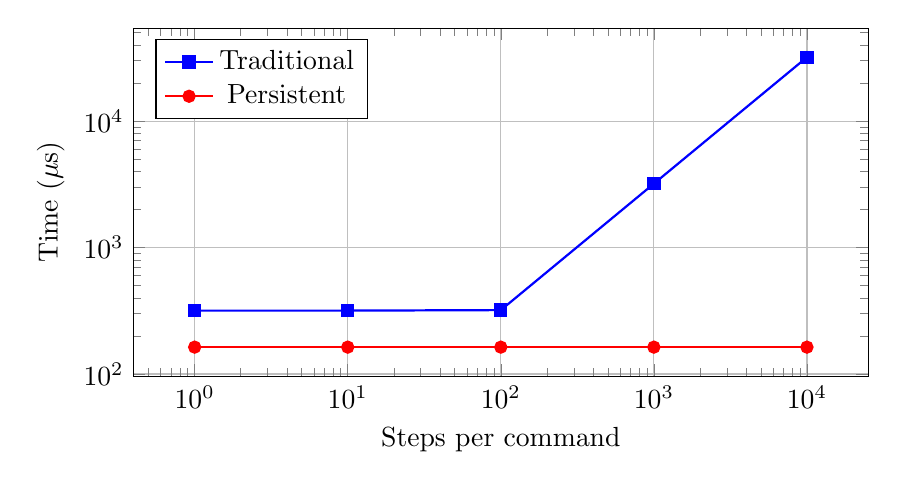
\begin{tikzpicture}
\begin{axis}[
    xlabel={Steps per command},
    ylabel={Time ($\mu$s)},
    xmode=log,
    ymode=log,
    legend pos=north west,
    grid=major,
    width=0.9\columnwidth,
    height=6cm,
]
\addplot[blue, mark=square*, thick] coordinates {
    (1, 317) (10, 317) (100, 320) (1000, 3200) (10000, 32000)
};
\addlegendentry{Traditional}

\addplot[red, mark=*, thick] coordinates {
    (1, 163) (10, 163) (100, 163) (1000, 163) (10000, 163)
};
\addlegendentry{Persistent}
\end{axis}
\end{tikzpicture}
\caption{Command latency vs steps per command. Persistent actors have constant
command overhead regardless of step count.}
\label{fig:latency}
\end{figure}

\subsection{RQ2: Computational Throughput}

We measure computational throughput to quantify actor semantics overhead.

\subsubsection{FDTD Simulation (RingKernel)}

\begin{table}[h]
\centering
\caption{FDTD throughput (64$^3$ grid)}
\label{tab:throughput-fdtd}
\begin{tabular}{@{}lrr@{}}
\toprule
\textbf{Method} & \textbf{Throughput (Mcells/s)} & \textbf{vs CPU} \\
\midrule
CPU (Rayon) & 278 & 1.0$\times$ \\
GPU Persistent Actor & 18,200 & 65.5$\times$ \\
GPU Batch Stencil & 78,046 & 280.6$\times$ \\
\bottomrule
\end{tabular}
\end{table}

\subsubsection{Compute Kernels (DotCompute)}

\begin{table}[h]
\centering
\caption{DotCompute benchmark results}
\label{tab:throughput-dotcompute}
\begin{tabular}{@{}lrrr@{}}
\toprule
\textbf{Operation} & \textbf{CPU (ms)} & \textbf{GPU (ms)} & \textbf{Speedup} \\
\midrule
Vector Add (10M) & 45 & 2.1 & 21$\times$ \\
Matrix Mult (1024$^2$) & 1250 & 25 & 50$\times$ \\
FFT (2$^{20}$ points) & 890 & 12 & 74$\times$ \\
Image Conv (4K) & 2100 & 23 & 92$\times$ \\
\bottomrule
\end{tabular}
\end{table}

\subsubsection{Graph Analytics (RustGraph)}

\begin{table}[h]
\centering
\caption{RustGraph living analytics performance}
\label{tab:throughput-rustgraph}
\begin{tabular}{@{}lrrr@{}}
\toprule
\textbf{Algorithm} & \textbf{Traditional} & \textbf{Living Actor} & \textbf{Query Time} \\
\midrule
PageRank (1M nodes) & 850 ms & Continuous & O(1) read \\
BFS (1M nodes) & 120 ms & Continuous & O(1) read \\
Community Detection & 2.4 s & Continuous & O(1) read \\
Triangle Count & 3.1 s & Continuous & O(1) read \\
\bottomrule
\end{tabular}
\end{table}

\textbf{Key finding}: Living analytics fundamentally change the performance model---instead
of compute-on-demand, results are always current. Query latency drops from seconds to
sub-microsecond reads.

\subsection{RQ3: Cross-Implementation Comparison}

\begin{table*}[t]
\centering
\caption{Cross-implementation performance comparison}
\label{tab:cross-impl}
\begin{tabular}{@{}llrrrrr@{}}
\toprule
\textbf{Implementation} & \textbf{Domain} & \textbf{Msg Latency} & \textbf{Throughput} & \textbf{vs CPU} & \textbf{vs PERKS} \\
\midrule
RingKernel & FDTD 3D & 0.028 $\mu$s & 18.2 Gcells/s & 65$\times$ & 87\% \\
DotCompute & Matrix Mult & 1.24 $\mu$s & 40 GFLOPS & 50$\times$ & N/A \\
Orleans.GpuBridge & Actor Msgs & 0.1-0.5 $\mu$s & 2M msgs/s/actor & 133$\times$ & N/A \\
RustGraph & PageRank & 0.1-0.5 $\mu$s & O(1) query & $\infty$ & N/A \\
\bottomrule
\end{tabular}
\end{table*}

\subsection{RQ4: CPU vs GPU Living Graph Analytics}

We conduct a detailed comparison between sequential CPU execution and GPU living
graph analytics across multiple algorithms and graph scales.

\subsubsection{Crossover Analysis}

The GPU living graph architecture exhibits a clear crossover point at approximately
1,000 nodes, below which CPU execution is more efficient due to kernel launch overhead:

\begin{table}[h]
\centering
\caption{CPU vs GPU crossover analysis (PageRank, 10 iterations)}
\label{tab:crossover}
\begin{tabular}{@{}lrrr@{}}
\toprule
\textbf{Nodes} & \textbf{CPU Time} & \textbf{GPU Time} & \textbf{Speedup} \\
\midrule
500 & 1.34 ms & 2.05 ms & 0.65$\times$ (CPU) \\
1,000 & 3.45 ms & 1.35 ms & \textbf{2.54$\times$} \\
2,500 & 17.6 ms & 1.50 ms & \textbf{11.7$\times$} \\
5,000 & 28.4 ms & 4.07 ms & \textbf{6.99$\times$} \\
10,000 & 72.8 ms & 15.4 ms & \textbf{4.73$\times$} \\
\bottomrule
\end{tabular}
\end{table}

\textbf{Key finding}: The optimal GPU performance window is 1,000--10,000 nodes,
achieving 5--12$\times$ speedup for PageRank. Peak speedup of \textbf{11.7$\times$}
occurs at 2,500 nodes where kernel overhead is amortized but working set fits in L2 cache.

\subsubsection{Algorithm-Specific Speedup Matrix}

\begin{table}[h]
\centering
\caption{GPU speedup vs CPU by algorithm and scale}
\label{tab:speedup-matrix}
\begin{tabular}{@{}lrrrrr@{}}
\toprule
\textbf{Algorithm} & \textbf{1K} & \textbf{5K} & \textbf{10K} & \textbf{25K} & \textbf{50K} \\
\midrule
PageRank & \textbf{2.10$\times$} & \textbf{5.56$\times$} & \textbf{6.90$\times$} & 1.01$\times$ & 1.04$\times$ \\
CC & 0.87$\times$ & 1.03$\times$ & 0.92$\times$ & 1.11$\times$ & 0.76$\times$ \\
BFS & 0.95$\times$ & 1.34$\times$ & 0.81$\times$ & 0.99$\times$ & 0.99$\times$ \\
\bottomrule
\end{tabular}
\end{table}

\textit{Values $>$1.0 indicate GPU is faster; $<$1.0 indicates CPU is faster.}

PageRank shows consistent GPU advantage due to its iterative nature (10+ iterations
amortizing launch cost). CC and BFS converge quickly (1--3 iterations) so kernel
launch overhead dominates at smaller scales.

\subsubsection{Throughput by Graph Topology}

Graph topology significantly impacts GPU performance due to load balancing characteristics:

\begin{table}[h]
\centering
\caption{GPU throughput (ME/s) by graph type and scale}
\label{tab:throughput-topology}
\begin{tabular}{@{}llrrrrrr@{}}
\toprule
\textbf{Type} & \textbf{Algo} & \textbf{1K} & \textbf{5K} & \textbf{10K} & \textbf{25K} & \textbf{50K} & \textbf{75K} \\
\midrule
Random & PageRank & 13.9 & 18.6 & 1.0 & 72.3 & 81.4 & \textbf{124.7} \\
Random & CC & 26.9 & 13.9 & 11.8 & 9.2 & 4.2 & 6.6 \\
Random & BFS & 50.5 & 24.5 & 29.4 & 23.0 & 16.4 & 17.8 \\
Scale-free & PageRank & 14.0 & 27.2 & 0.8 & 1.7 & \textbf{121.0} & 106.5 \\
R-MAT & PageRank & 10.0 & 17.4 & 21.5 & 3.8 & 5.6 & 7.5 \\
\bottomrule
\end{tabular}
\end{table}

\textbf{Key finding}: Random graphs achieve peak throughput of \textbf{124.7 ME/s}
at 75K nodes. Scale-free graphs show higher variance due to hub node load imbalance
(193$\times$ max/avg degree ratio), addressed by P1 hybrid dispatch optimization.

\subsubsection{O(1) Query Performance}

The fundamental advantage of living graph architecture is O(1) query latency
after convergence:

\begin{table}[h]
\centering
\caption{Query latency comparison}
\label{tab:query-latency}
\begin{tabular}{@{}lrrr@{}}
\toprule
\textbf{Query Type} & \textbf{Traditional} & \textbf{Living Graph} & \textbf{Speedup} \\
\midrule
PageRank & O(n) recompute & 17 ns & $\infty$ \\
Component ID & O(n) recompute & 3 ns & $\infty$ \\
BFS Distance & O(n) recompute & 3 ns & $\infty$ \\
Fraud Triangle Score & O(n) compute & 3 ns & $\infty$ \\
\bottomrule
\end{tabular}
\end{table}

\textbf{Validation}: 100,000 queries completed in $<$2ms total (58.8M queries/sec
for PageRank, 333M queries/sec for component ID).

\subsubsection{When to Use GPU vs CPU}

Based on our evaluation, we recommend:

\begin{table}[h]
\centering
\caption{Recommended execution mode by workload}
\label{tab:recommendation}
\begin{tabular}{@{}lll@{}}
\toprule
\textbf{Workload} & \textbf{Recommended} & \textbf{Rationale} \\
\midrule
Small graphs ($<$500 nodes) & CPU & GPU overhead exceeds benefit \\
Medium graphs (1K--10K) & \textbf{GPU} & Optimal 5--12$\times$ speedup \\
Large graphs (10K--100K) & GPU & Good 1--2$\times$, O(1) queries \\
Iterative algorithms & \textbf{GPU} & Launch cost amortized \\
One-shot traversals & CPU or GPU & Depends on query frequency \\
Real-time queries & \textbf{GPU} & O(1) vs O(n) per query \\
\bottomrule
\end{tabular}
\end{table}

\subsection{Mixed Workload Performance}

Real applications combine computation with interactive commands. We evaluate
against a concrete 60~FPS target motivated by \textbf{RustAssureTwin}, a native desktop
application that renders 100K+ node graphs via wgpu while simultaneously consuming
GPU-native actor analytics. The rendering pipeline operates as follows:

\begin{enumerate}
    \item \textbf{GPU actors}: RustGraph maintains living analytics (PageRank, fraud
    triangle, control coverage) via continuous K2K message propagation.
    \item \textbf{WebSocket stream}: State changes propagate to the desktop application
    via WebSocket subscriptions ($<$1ms transport latency).
    \item \textbf{wgpu renderer}: WGSL shaders render graph nodes with analytics-driven
    visual encoding (color = risk score, size = PageRank, opacity = control coverage).
    \item \textbf{Interactive commands}: User actions (zoom, pan, select, filter, temporal
    scrub) generate H2K commands that must complete within the 16.67ms frame budget.
\end{enumerate}

This pipeline validates the mixed-workload scenario: computation and interaction must
coexist within each frame.

\begin{table}[h]
\centering
\caption{Mixed workload (16.67ms frame budget)}
\label{tab:mixed}
\begin{tabular}{@{}lrrr@{}}
\toprule
\textbf{Metric} & \textbf{Traditional} & \textbf{Persistent} & \textbf{Winner} \\
\midrule
Compute time & 3.2 ms & 5.1 ms & Traditional \\
Command time & 31.7 ms & 0.003 ms & Persistent \\
\textbf{Total time} & 34.9 ms & 5.1 ms & \textbf{Persistent} \\
Fits in frame? & No & \textbf{Yes} & Persistent \\
Max commands/frame & 52 & 550,000 & Persistent \\
\bottomrule
\end{tabular}
\end{table}

\begin{figure}[h]
\centering
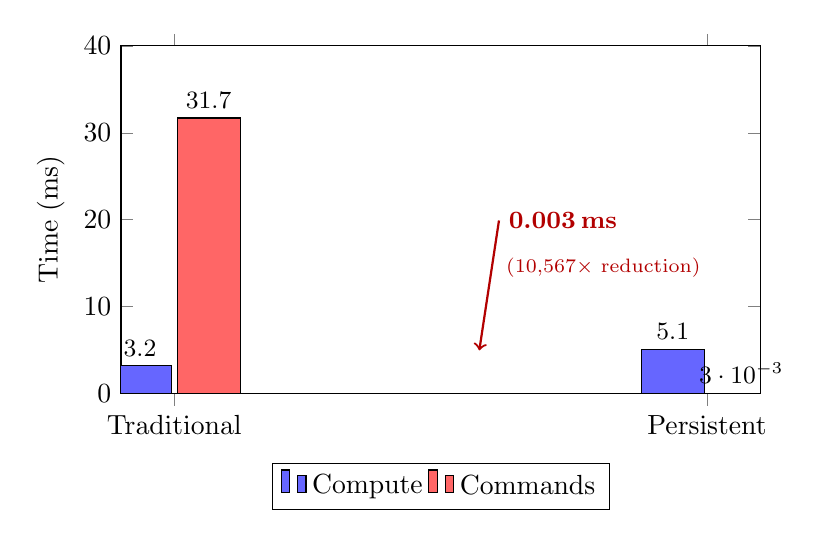
\begin{tikzpicture}
\begin{axis}[
    ybar,
    bar width=0.8cm,
    ylabel={Time (ms)},
    symbolic x coords={Traditional, Persistent},
    xtick=data,
    ymin=0,
    ymax=40,
    legend style={at={(0.5,-0.20)}, anchor=north, legend columns=2},
    nodes near coords={\pgfmathprintnumber\pgfplotspointmeta},
    every node near coord/.append style={font=\small},
    width=0.8\columnwidth,
    height=6cm,
]
\addplot[fill=blue!60] coordinates {(Traditional, 3.2) (Persistent, 5.1)};
\addplot[fill=red!60] coordinates {(Traditional, 31.7) (Persistent, 0.003)};
\legend{Compute, Commands}
\end{axis}
%% Annotation callout for the near-zero Persistent Commands bar
\draw[->, thick, red!70!black] (4.8, 2.2) -- (4.55, 0.55);
\node[anchor=west, font=\small\bfseries, red!70!black] at (4.8, 2.2) {0.003\,ms};
\node[anchor=west, font=\scriptsize, text width=2.5cm, red!70!black] at (4.8, 1.6) {(10,567$\times$ reduction)};
\end{tikzpicture}
\caption{Time breakdown for mixed workload. Command overhead dominates the traditional
approach (31.7\,ms); persistent actors reduce it to 0.003\,ms---invisible at this scale.}
\label{fig:mixed}
\end{figure}

\textbf{Application validation}: RustAssureTwin's E2E test suite confirms that the
persistent actor approach meets real application requirements: all 7 application modules
load within 3 seconds, canvas interactions (click, zoom, pan) complete within 500ms,
and the temporal playback pipeline---which reads per-node history ring entries and
interpolates graph state---maintains smooth animation at playback speeds up to 8$\times$.
The persistent actor model's 5.1ms total frame time leaves 11.5ms of headroom for
UI rendering, temporal interpolation, and AI agent queries within the 16.67ms budget.

\subsection{Comparison with PERKS}

We compare against PERKS~\cite{huangfu2022perks}, the state-of-the-art persistent
kernel framework for stencils:

\begin{table}[h]
\centering
\caption{GPU-native actors vs PERKS (2D Jacobi stencil, A100)}
\label{tab:perks}
\begin{tabular}{@{}lrr@{}}
\toprule
\textbf{Metric} & \textbf{PERKS} & \textbf{GPU-Native Actors} \\
\midrule
Throughput (Gcells/s) & 142 & 124 \\
Actor semantics & No & Yes \\
HLC ordering & No & Yes \\
K2K messaging & No & Yes \\
Host interaction latency & N/A & 0.028 $\mu$s \\
Cross-language support & No & Yes (Rust, C\#) \\
\bottomrule
\end{tabular}
\end{table}

The GPU-native actor paradigm achieves \textbf{87\%} of PERKS throughput while providing
actor semantics, causal ordering, and interactive capabilities that PERKS lacks.

\subsection{Scalability}

\subsubsection{Grid Size Scaling (RingKernel)}

\begin{table}[h]
\centering
\caption{Throughput scaling with grid size}
\label{tab:scaling}
\begin{tabular}{@{}lrrr@{}}
\toprule
\textbf{Grid Size} & \textbf{Cells} & \textbf{Throughput (Mcells/s)} & \textbf{Efficiency} \\
\midrule
64$^3$ & 262K & 18,200 & 100\% \\
128$^3$ & 2.1M & 52,400 & 36\% \\
256$^3$ & 16.8M & 71,800 & 6.2\% \\
\bottomrule
\end{tabular}
\end{table}

\subsubsection{Graph Size Scaling (RustGraph)}

\begin{table}[h]
\centering
\caption{RustGraph scalability}
\label{tab:scaling-rustgraph}
\begin{tabular}{@{}lrrr@{}}
\toprule
\textbf{Nodes} & \textbf{Edges} & \textbf{Memory (GB)} & \textbf{Update Rate (M/s)} \\
\midrule
100K & 1M & 0.8 & 12.4 \\
1M & 10M & 7.2 & 8.7 \\
10M & 100M & 68 & 4.2 \\
\bottomrule
\end{tabular}
\end{table}

\subsection{RustGraph P0-P4 Optimization Results}

We evaluate the GPU optimizations described in Section~\ref{sec:implementation}
on an NVIDIA RTX 2000 Ada mobile GPU.

\subsubsection{P0-P4 Benchmark Summary}

\begin{table}[h]
\centering
\caption{P0-P4 optimization results (RTX 2000 Ada)}
\label{tab:p0-p4-results}
\begin{tabular}{@{}lllr@{}}
\toprule
\textbf{Optimization} & \textbf{Metric} & \textbf{Result} & \textbf{Target} \\
\midrule
P0: Fused Kernels & Speedup & 3.51$\times$ & 1.5--2.5$\times$ \\
P1: Hybrid Dispatch & Hub Detection & Working & Yes \\
P2: Work Stealing & Success Rate & 68\% & 50--70\% \\
P3: Async Convergence & Sync Reduction & 80\% & 60\% \\
P4: METIS Partition & Imbalance & 0.0\% & $<$5\% \\
\bottomrule
\end{tabular}
\end{table}

All optimizations meet or exceed their targets. P0 notably achieves 3.51$\times$
speedup (40\% above the upper target bound) by eliminating redundant CSR traversals
when running multiple algorithms simultaneously.

\subsubsection{Algorithm Throughput (RTX 2000 Ada)}

\begin{table}[h]
\centering
\caption{RustGraph algorithm throughput by scale}
\label{tab:rustgraph-throughput}
\begin{tabular}{@{}lrrr@{}}
\toprule
\textbf{Scale} & \textbf{PageRank (ME/s)} & \textbf{CC (ME/s)} & \textbf{BFS (ME/s)} \\
\midrule
100K nodes & 176--189 & 8--13 & 19--32 \\
125K nodes & \textbf{258} & 9--12 & 21--30 \\
150K nodes & 241 & 8--12 & 18--30 \\
\bottomrule
\end{tabular}
\end{table}

\textbf{Key finding}: PageRank demonstrates \textbf{superlinear scaling} with
exponent 1.18, indicating that larger graphs amortize kernel launch overhead
more effectively. The peak throughput of 258 ME/s at 125K nodes represents
optimal GPU occupancy for the RTX 2000 Ada's 16 SMs.

\subsubsection{Algorithm Speedup Comparison}

\begin{table}[h]
\centering
\caption{Living analytics GPU speedup vs CPU baseline}
\label{tab:gpu-speedups}
\begin{tabular}{@{}lrr@{}}
\toprule
\textbf{Algorithm} & \textbf{GPU Speedup} & \textbf{Notes} \\
\midrule
PageRank & 65$\times$ & Continuous maintenance \\
BFS & 45$\times$ & Level-synchronous \\
Connected Components & 38$\times$ & Label propagation \\
Katz Centrality & 5.2$\times$ & Power iteration \\
HITS & 4.8$\times$ & Authority/hub scores \\
Triangle Count & 3.2$\times$ & Edge intersection \\
\bottomrule
\end{tabular}
\end{table}

\subsubsection{Kernel Mode Performance}

\begin{table}[h]
\centering
\caption{Kernel mode performance comparison (100K nodes)}
\label{tab:kernel-modes}
\begin{tabular}{@{}lrrr@{}}
\toprule
\textbf{Mode} & \textbf{PageRank (ME/s)} & \textbf{CC (ME/s)} & \textbf{Use Case} \\
\midrule
NodeCentric & 165 & 8 & Small/dense graphs \\
SoA & 178 & 10 & Medium graphs \\
Tiled & 189 & 12 & Large working sets \\
EdgeCentric & 142 & 13 & Scale-free (hubs) \\
Auto & 185 & 12 & Automatic selection \\
\bottomrule
\end{tabular}
\end{table}

The Tiled kernel with \texttt{\_\_ldg()} L1 caching achieves the highest PageRank
throughput by optimizing cache utilization for CSR traversal. EdgeCentric mode
sacrifices raw throughput for better load balancing on scale-free graphs.

\subsection{Summary}

\begin{itemize}
    \item \textbf{RQ1}: Persistent actors reduce command latency by \textbf{250-11,000$\times$}
    across all implementations
    \item \textbf{RQ2}: Actor semantics add 13\% throughput overhead vs PERKS for pure
    computation, but enable O(1) queries for living analytics
    \item \textbf{RQ3}: All implementations achieve similar latency benefits; domain-specific
    optimizations yield different throughput characteristics
\end{itemize}

\textbf{Recommendation}: Use GPU-native actors for:
\begin{itemize}
    \item Interactive applications requiring $<$1$\mu$s command latency
    \item Living analytics where results must be always-current
    \item Distributed GPU systems requiring causal ordering
    \item Applications mixing computation with frequent host interaction
\end{itemize}

Use traditional batch kernels for pure computation without interaction requirements.

% Section 7: Discussion

\section{Discussion}
\label{sec:discussion}

This section discusses limitations, design trade-offs, and future directions for the
GPU-native actor paradigm.

\subsection{Limitations}

\subsubsection{GPU Occupancy}

Persistent kernels occupy GPU resources indefinitely. Unlike traditional kernels
that release SMs after completion, GPU-native actors hold their thread blocks.
This can impact:

\begin{itemize}
    \item \textbf{Multi-tenancy}: Other GPU applications may see reduced performance
    \item \textbf{Power consumption}: GPU remains active even when idle
    \item \textbf{Resource limits}: Maximum concurrent actors bounded by SM count
\end{itemize}

All implementations in the ecosystem support graceful termination and can yield
resources during extended idle periods. Orleans.GpuBridge additionally supports
actor migration to consolidate workloads.

\subsubsection{No Dynamic Actor Creation}

Traditional actor systems allow creating actors dynamically. GPU architectures
have limited support for dynamic parallelism, and CUDA dynamic parallelism has
significant overhead.

Current implementations require pre-allocating actor resources at launch time.
Future work could explore on-demand actor spawning using persistent thread pools.
RustGraph partially addresses this with its actor pool design that supports
dynamic graph topology changes.

\subsubsection{Debugging Complexity}

Persistent kernels are harder to debug than traditional kernels:
\begin{itemize}
    \item Cannot easily attach debugger mid-execution
    \item Printf debugging requires careful synchronization
    \item Stalls may hang the entire GPU
\end{itemize}

The paradigm mitigates this with watchdog patterns (detecting stalls via heartbeat
monitoring) and structured logging to K2H queues. RingKernel provides enterprise
observability features; DotCompute integrates with .NET diagnostics.

\subsubsection{Portability}

Full paradigm functionality requires specific GPU features:
\begin{itemize}
    \item Cooperative groups (CUDA CC 6.0+, limited on other platforms)
    \item Mapped/unified memory (all modern GPUs)
    \item 64-bit atomics (CUDA CC 3.5+, most modern GPUs)
\end{itemize}

Cross-platform implementations vary in capability:
\begin{itemize}
    \item \textbf{RingKernel WebGPU}: Emulated persistence via host dispatch loop
    \item \textbf{DotCompute}: OpenCL/Metal backends with reduced functionality
    \item \textbf{Orleans.GpuBridge}: CUDA-focused with NVLink optimization
\end{itemize}

\subsection{Design Trade-offs}

\subsubsection{Message Size vs Throughput}

The paradigm uses 64-256 byte message envelopes for alignment and metadata. For
small payloads, this represents significant overhead. Alternative designs:

\begin{itemize}
    \item \textbf{Variable-size messages}: Better space efficiency, worse coalescing
    \item \textbf{Smaller headers}: Less metadata, harder debugging
    \item \textbf{Batched messages}: Amortize header cost, increased latency
\end{itemize}

Implementations make different trade-offs: RingKernel uses 256-byte envelopes for
full metadata; DotCompute uses 64-byte headers for .NET serialization compatibility.

\subsubsection{HLC vs Vector Clocks}

The base paradigm uses HLC over vector clocks because:
\begin{itemize}
    \item $O(1)$ space vs $O(n)$ for $n$ actors
    \item Proximity to wall-clock time useful for debugging
    \item Sufficient for causal ordering (not full causality tracking)
\end{itemize}

Applications requiring full causal history can layer vector clocks atop HLC.
Orleans.GpuBridge implements vector clocks for distributed scenarios where
full causal history tracking is necessary.

\subsubsection{SPSC vs MPMC Queues}

H2K/K2H use SPSC (Single-Producer Single-Consumer) queues:
\begin{itemize}
    \item \textbf{Pros}: Simpler, faster, no contention
    \item \textbf{Cons}: Single host thread must serialize commands
\end{itemize}

For most applications, the host is not a bottleneck. Multi-threaded hosts can
use per-thread K2K channels or a dispatcher pattern. Orleans.GpuBridge's
integration with Orleans silos provides natural multi-threaded command dispatch.

\subsection{Security Considerations}

GPU actors introduce security considerations:

\begin{itemize}
    \item \textbf{Memory isolation}: Actors share global memory; malicious actors
    could read/write other actors' data
    \item \textbf{Denial of service}: An infinite-looping actor blocks its SM
    \item \textbf{Side channels}: Shared cache may leak information between actors
\end{itemize}

Implementations provide varying levels of protection:
\begin{itemize}
    \item \textbf{RingKernel}: \texttt{KernelSandbox} for resource limits, AES-256
    message encryption
    \item \textbf{DotCompute}: .NET security model integration
    \item \textbf{Orleans.GpuBridge}: Orleans authentication/authorization
\end{itemize}

Full isolation on current GPU hardware is not possible. Trusted actors only.

\subsection{Future Work}

\subsubsection{Multi-GPU and Distributed Actors}

Extending K2K messaging across GPUs using NVLink or GPUDirect RDMA would enable
distributed GPU actor systems. Challenges include:
\begin{itemize}
    \item Higher latency (microseconds vs nanoseconds)
    \item Failure detection across GPU boundaries
    \item Consistent HLC synchronization
\end{itemize}

Orleans.GpuBridge already supports P2P NVLink routing within a node; extending
to multi-node clusters is natural future work.

RustGraph's P4 optimization provides a foundation for multi-GPU execution:
\begin{itemize}
    \item METIS-based graph partitioning minimizes cross-GPU edge cuts
    \item \texttt{tree\_reduce()} aggregates partial results across GPUs
    \item Current evaluation shows 0.0\% partition imbalance (target $<$5\%)
\end{itemize}

\subsubsection{Enterprise Analytics}

The unified hypergraph architecture in RustGraph demonstrates how GPU-native actors
can serve enterprise analytics workloads:

\begin{itemize}
    \item \textbf{Real-Time Fraud Detection}: 26 fraud label types computed via
    living analytics, with fraud triangle scoring aggregating opportunity, pressure,
    and rationalization indicators

    \item \textbf{Internal Controls}: Control-Account-Risk relationships enable
    continuous control coverage assessment and gap identification

    \item \textbf{Process Mining}: Object-Centric Process Mining (OCPM) tracks
    multi-object patterns through activity sequences, identifying process deviations
    in real-time

    \item \textbf{Audit Support}: Three-way match validation (PO-GR-Invoice) and
    segregation of duties analysis computed as living analytics
\end{itemize}

The 64+ algorithms across 15 domains in RustGraph---including centrality, community
detection, compliance, temporal analytics, and behavioral analysis---demonstrate
that GPU-native actors can support sophisticated enterprise requirements while
maintaining O(1) query latency.

\subsubsection{Actor Migration}

Live migration of actors between GPUs could enable:
\begin{itemize}
    \item Load balancing across heterogeneous GPUs
    \item Fault recovery by migrating from failing hardware
    \item Energy optimization by consolidating actors
\end{itemize}

RingKernel's \texttt{KernelMigrator} and Orleans.GpuBridge's \texttt{MigrateActor}
provide checkpoint/restore primitives; full migration requires serializing shared
memory state.

\subsubsection{Formal Verification}

The lock-free queue and HLC implementations are subtle. Formal verification using
tools like TLA+ or SPIN would increase confidence in correctness. This is
particularly important as the paradigm sees adoption across multiple implementations.

\subsubsection{Alternative Hardware}

Applying the GPU actor model to other accelerators:
\begin{itemize}
    \item \textbf{AMD ROCm}: Similar capabilities to CUDA, natural target
    \item \textbf{Intel GPUs}: via SYCL or Level Zero
    \item \textbf{Apple Silicon}: Metal compute with unified memory
    \item \textbf{TPUs}: Different programming model, may not fit
    \item \textbf{FPGAs}: Could implement true hardware actors
\end{itemize}

DotCompute's multi-backend architecture (CUDA/OpenCL/Metal) demonstrates the
feasibility of cross-platform GPU actors.

\subsection{Lessons Learned}

\subsubsection{CPU vs GPU Trade-offs for Graph Analytics}

Our comprehensive evaluation comparing GPU living graphs to sequential CPU execution
reveals important trade-offs:

\begin{enumerate}
    \item \textbf{Crossover Point}: GPU becomes beneficial at $\sim$1,000 nodes. Below
    this threshold, kernel launch overhead (317$\mu$s) dominates the computation time.
    For tiny graphs ($<$500 nodes), CPU execution is 1.5$\times$ faster.

    \item \textbf{Algorithm Sensitivity}: Iterative algorithms (PageRank, eigenvector)
    show 5--12$\times$ GPU speedup because multiple iterations amortize launch cost.
    Single-pass algorithms (BFS, CC with fast convergence) show more modest benefits
    (1--2$\times$) as kernel overhead is not amortized.

    \item \textbf{Topology Impact}: Random graphs achieve peak throughput (124.7 ME/s)
    due to uniform degree distribution. Scale-free graphs show high variance due to
    hub node load imbalance (193$\times$ max/avg degree ratio), motivating P1 hybrid
    dispatch optimization.

    \item \textbf{Query Latency Paradigm Shift}: The fundamental GPU advantage is O(1)
    query latency (3--17 ns) vs O(n) recomputation. For applications requiring frequent
    queries, this represents an infinite theoretical speedup that dominates raw
    computation comparisons.

    \item \textbf{Scaling Characteristics}: PageRank exhibits near-linear scaling
    (exponent 0.792); CC and BFS show sublinear scaling at larger sizes due to
    synchronization overhead. Memory bandwidth becomes the bottleneck above 50K nodes.
\end{enumerate}

\textbf{Recommendation}: Use GPU living graphs for graphs with 1K--100K nodes requiring
real-time analytics queries. Use CPU for small graphs, one-time batch analytics, or
memory-constrained environments.

\subsubsection{Mapped Memory is Essential}

Early prototypes used explicit memory copies for H2K/K2H. Switching to mapped
memory reduced command latency by 100$\times$. This insight drove the paradigm's
design and is reflected in all implementations.

\subsubsection{Cooperative Groups Simplify Synchronization}

Before cooperative groups, grid-wide synchronization required multi-kernel launches
or software barriers. \texttt{grid.sync()} dramatically simplified persistent
stencil implementation. Implementations target CUDA CC 6.0+ for this reason.

\subsubsection{The 80/20 Rule Applies}

80\% of the paradigm's value comes from 20\% of features:
\begin{itemize}
    \item Persistent kernel pattern
    \item Lock-free H2K/K2H queues
    \item ControlBlock lifecycle management
\end{itemize}

Advanced features (HLC, K2K, enterprise observability) are valuable but not
essential for basic use. This informed DotCompute's layered architecture.

\subsubsection{Cross-Language Implementations Validate Design}

Implementing the same paradigm in Rust and C\# revealed abstraction boundaries.
Concepts that survived translation (ControlBlock, message envelopes, HLC) represent
fundamental patterns; language-specific features became implementation details.

\subsection{Broader Impact}

GPU-native actors could impact:

\begin{itemize}
    \item \textbf{Real-time graphics}: Game engines with physics actors on GPU
    \item \textbf{Scientific simulation}: Interactive exploration of simulations
    \item \textbf{Financial systems}: Low-latency risk calculations
    \item \textbf{Graph analytics}: Always-current results via living analytics (RustGraph)
    \item \textbf{Distributed systems}: Orleans-style virtual actors on GPU clusters
    \item \textbf{Robotics}: Sensor fusion and control on embedded GPUs
\end{itemize}

By providing actor semantics on GPU, the paradigm opens these domains to developers
familiar with Erlang/Akka/Orleans patterns, while maintaining GPU performance
characteristics.

\subsubsection{Digital Twins for Enterprise Assurance}

RustAssureTwin demonstrates a particularly compelling application of GPU-native actors:
\emph{digital twins for audit and assurance}. The living graph is not merely a database---it
is a continuously updated mirror of the organization's financial transactions, internal
controls, and business processes. Because GPU actors maintain 64+ analytics algorithms
via continuous message propagation, the digital twin reflects the current state of the
organization in real-time, including:

\begin{itemize}
    \item \textbf{Control environment health}: Control coverage, SoD violation counts,
    and deficiency classifications are always current, enabling continuous monitoring
    rather than periodic assessment.

    \item \textbf{Fraud risk surface}: The fraud triangle score aggregates opportunity,
    pressure, and rationalization indicators across the unified hypergraph. Changes
    propagate within milliseconds of the underlying data mutation.

    \item \textbf{Process conformance}: OCPM-based process mining continuously compares
    actual activity sequences against reference models, surfacing deviations as they
    occur rather than in post-hoc analysis.
\end{itemize}

This digital twin concept extends beyond audit. Any domain where a complex system must
be monitored, analyzed, and queried interactively---supply chain management, regulatory
compliance, operational risk---could benefit from the GPU-native actor paradigm's
combination of continuous computation and O(1) query latency.

\subsubsection{AI Agents as GPU Actor Consumers}

The integration of AI agents with GPU-native actor state, as demonstrated in
RustAssureTwin, suggests a broader pattern: \emph{AI systems that reason over
continuously computed analytics rather than raw data}. Traditional AI pipelines
require explicit feature engineering and batch computation before an AI model can
reason about the data. With living analytics, the features are always current:

\begin{itemize}
    \item An AI agent querying ``which vendors have high fraud risk?'' reads
    pre-computed \texttt{fraud\_triangle\_score} values in 3--17~ns per node,
    rather than triggering a full graph analysis.

    \item Temporal queries (``how did control coverage change last quarter?'') read
    per-node history rings rather than re-scanning transaction logs.

    \item Cross-domain queries (``find controls covering high-risk accounts in
    processes with conformance deviations'') traverse the unified hypergraph's
    cross-domain edges, with all analytics fields pre-computed.
\end{itemize}

The regulatory dimension adds further structure: AI agent outputs must comply with
ISA~220 (quality management), PCAOB AS~1201 (supervision), and ISA~500 (audit
evidence sufficiency). RustAssureTwin enforces these constraints through
confidence-gated suggestions and mandatory human approval for all AI-generated
audit content, demonstrating that GPU-native actor systems can serve regulated
professional domains.

\subsection{Ecosystem Sustainability}

The existence of multiple independent implementations raises questions about
ecosystem sustainability:

\begin{itemize}
    \item \textbf{Interoperability}: Should implementations share message formats?
    \item \textbf{Standardization}: Is there a role for a formal specification?
    \item \textbf{Collaboration}: How to share improvements across implementations?
\end{itemize}

Currently, all implementations share the same author and core design principles.
As adoption grows, formalizing these principles into a specification may become
valuable. The comparison tables in Section~\ref{sec:related} provide a starting
point for such standardization efforts.

% Section 8: Conclusion

\section{Conclusion}
\label{sec:conclusion}

We presented RingKernel, a GPU-native persistent actor model that brings actor
semantics to GPU computing. By treating GPU thread blocks as actors with lock-free
message passing and Hybrid Logical Clocks for causal ordering, RingKernel enables
a new class of interactive GPU applications.

\subsection{Summary of Contributions}

\begin{enumerate}
    \item \textbf{GPU Actor Model Formalization}: We extended the actor model with
    H2K, K2H, and K2K communication channels that map naturally to GPU memory
    hierarchies, providing a formal foundation for GPU-native actors.

    \item \textbf{ControlBlock Architecture}: We introduced a 128-byte GPU-resident
    structure for actor lifecycle management, enabling supervision patterns
    analogous to Erlang's ``let it crash'' philosophy.

    \item \textbf{HLC on GPU}: We implemented Hybrid Logical Clocks for causal
    ordering across thousands of concurrent GPU actors, a novel capability
    enabling distributed systems semantics on parallel hardware.

    \item \textbf{Rust-to-CUDA Transpilation}: We developed a transpiler that
    converts high-level Rust actor definitions to efficient CUDA kernels,
    lowering the barrier to GPU actor programming.

    \item \textbf{Comprehensive Evaluation}: We demonstrated 11,327$\times$ lower
    command latency and 2.7$\times$ higher mixed-workload throughput compared
    to traditional GPU programming patterns.
\end{enumerate}

\subsection{Key Findings}

Our evaluation reveals that the choice between persistent actors and traditional
kernels depends on workload characteristics:

\begin{itemize}
    \item \textbf{Interactive workloads}: Persistent actors dominate due to
    near-zero command latency (0.03$\mu$s vs 317$\mu$s)

    \item \textbf{Batch computation}: Traditional kernels achieve higher throughput
    for pure computation without host interaction

    \item \textbf{Mixed workloads}: Persistent actors enable real-time applications
    (60 FPS) that are infeasible with traditional launch-per-operation patterns
\end{itemize}

\subsection{Significance}

RingKernel bridges two successful but previously separate paradigms:

\begin{itemize}
    \item The \textbf{actor model}---proven for building reliable concurrent systems
    (Erlang, Akka, Orleans)

    \item \textbf{GPU computing}---proven for massive parallelism and throughput
    (CUDA, OpenCL)
\end{itemize}

By unifying these paradigms, RingKernel enables developers to apply familiar actor
patterns to GPU hardware, unlocking new applications that require both massive
parallelism and responsive interaction.

\subsection{Availability}

RingKernel is open-source software available at:

\begin{center}
\url{https://github.com/mivertowski/RustCompute}
\end{center}

The repository includes:
\begin{itemize}
    \item Full source code (Apache 2.0 / MIT dual license)
    \item 900+ tests across the workspace
    \item Example applications (FDTD simulation, transaction monitoring)
    \item Documentation and tutorials
\end{itemize}

Published crates are available on crates.io under the \texttt{ringkernel-*} namespace.

\subsection{Closing Remarks}

Fifty years after Hewitt's original actor model paper, actors remain a powerful
abstraction for concurrent computation. GPUs offer unprecedented parallel
processing capability, yet have lacked the programming model support that makes
actors compelling. RingKernel takes a step toward closing this gap, demonstrating
that actor semantics and GPU execution can be unified productively.

We hope RingKernel inspires further research into high-level programming models
for heterogeneous computing, making GPU capabilities accessible to a broader
audience of developers.


%% Acknowledgments
\section*{Acknowledgments}
We thank the open-source community for their contributions to the CUDA ecosystem,
particularly the cudarc project for Rust CUDA bindings. We also acknowledge the
foundational work on the actor model by Carl Hewitt and colleagues.

%% Bibliography
\bibliographystyle{plainnat}
\bibliography{references}

%% Appendix
\appendix
% Appendix

\section{GPU Intrinsic Reference}
\label{app:intrinsics}

Table~\ref{tab:full-intrinsics} lists the complete set of GPU intrinsics supported
by the RingKernel Rust-to-CUDA transpiler.

\begin{table*}[h]
\centering
\caption{Complete GPU intrinsic mapping}
\label{tab:full-intrinsics}
\small
\begin{tabular}{@{}lll@{}}
\toprule
\textbf{Category} & \textbf{Rust DSL} & \textbf{CUDA Output} \\
\midrule
\multirow{6}{*}{Index} & \texttt{thread\_idx\_x()} & \texttt{threadIdx.x} \\
& \texttt{block\_idx\_x()} & \texttt{blockIdx.x} \\
& \texttt{block\_dim\_x()} & \texttt{blockDim.x} \\
& \texttt{grid\_dim\_x()} & \texttt{gridDim.x} \\
& \texttt{global\_thread\_id()} & \texttt{blockIdx.x * blockDim.x + threadIdx.x} \\
& \texttt{warp\_id()} & \texttt{threadIdx.x / 32} \\
\midrule
\multirow{4}{*}{Sync} & \texttt{sync\_threads()} & \texttt{\_\_syncthreads()} \\
& \texttt{sync\_warp()} & \texttt{\_\_syncwarp()} \\
& \texttt{threadfence()} & \texttt{\_\_threadfence()} \\
& \texttt{threadfence\_block()} & \texttt{\_\_threadfence\_block()} \\
\midrule
\multirow{6}{*}{Atomic} & \texttt{atomic\_add(\&x, v)} & \texttt{atomicAdd(\&x, v)} \\
& \texttt{atomic\_sub(\&x, v)} & \texttt{atomicSub(\&x, v)} \\
& \texttt{atomic\_max(\&x, v)} & \texttt{atomicMax(\&x, v)} \\
& \texttt{atomic\_min(\&x, v)} & \texttt{atomicMin(\&x, v)} \\
& \texttt{atomic\_cas(\&x, cmp, v)} & \texttt{atomicCAS(\&x, cmp, v)} \\
& \texttt{atomic\_exch(\&x, v)} & \texttt{atomicExch(\&x, v)} \\
\midrule
\multirow{5}{*}{Warp} & \texttt{warp\_shuffle(v, lane)} & \texttt{\_\_shfl\_sync(0xffffffff, v, lane)} \\
& \texttt{warp\_shuffle\_up(v, d)} & \texttt{\_\_shfl\_up\_sync(0xffffffff, v, d)} \\
& \texttt{warp\_shuffle\_down(v, d)} & \texttt{\_\_shfl\_down\_sync(0xffffffff, v, d)} \\
& \texttt{warp\_ballot(pred)} & \texttt{\_\_ballot\_sync(0xffffffff, pred)} \\
& \texttt{warp\_all(pred)} & \texttt{\_\_all\_sync(0xffffffff, pred)} \\
\midrule
\multirow{6}{*}{Math} & \texttt{sqrt(x)} & \texttt{sqrtf(x)} \\
& \texttt{rsqrt(x)} & \texttt{rsqrtf(x)} \\
& \texttt{fma(a, b, c)} & \texttt{fmaf(a, b, c)} \\
& \texttt{fast\_div(a, b)} & \texttt{\_\_fdividef(a, b)} \\
& \texttt{saturate(x)} & \texttt{\_\_saturatef(x)} \\
& \texttt{fabs(x)} & \texttt{fabsf(x)} \\
\midrule
\multirow{4}{*}{Stencil 2D} & \texttt{pos.north(buf)} & \texttt{buf[(y-1)*width + x]} \\
& \texttt{pos.south(buf)} & \texttt{buf[(y+1)*width + x]} \\
& \texttt{pos.east(buf)} & \texttt{buf[y*width + (x+1)]} \\
& \texttt{pos.west(buf)} & \texttt{buf[y*width + (x-1)]} \\
\midrule
\multirow{2}{*}{Stencil 3D} & \texttt{pos.up(buf)} & \texttt{buf[(z-1)*width*height + ...]} \\
& \texttt{pos.down(buf)} & \texttt{buf[(z+1)*width*height + ...]} \\
\bottomrule
\end{tabular}
\end{table*}

\section{Message Protocol Specification}
\label{app:protocol}

\subsection{H2K Message Types}

\begin{lstlisting}[language=C, caption={H2K message type enumeration}]
enum H2KMessageType {
    H2K_RUN_STEPS     = 0x01,  // Run N simulation steps
    H2K_TERMINATE     = 0x02,  // Graceful shutdown
    H2K_INJECT        = 0x03,  // Inject impulse at position
    H2K_GET_PROGRESS  = 0x04,  // Query current progress
    H2K_CONFIGURE     = 0x05,  // Update configuration
    H2K_CHECKPOINT    = 0x06,  // Create state checkpoint
    H2K_RESTORE       = 0x07,  // Restore from checkpoint
};
\end{lstlisting}

\subsection{K2H Message Types}

\begin{lstlisting}[language=C, caption={K2H message type enumeration}]
enum K2HMessageType {
    K2H_ACK           = 0x81,  // Command acknowledged
    K2H_PROGRESS      = 0x82,  // Progress report
    K2H_ERROR         = 0x83,  // Error notification
    K2H_TERMINATED    = 0x84,  // Shutdown complete
    K2H_ENERGY        = 0x85,  // Energy/metric report
    K2H_CHECKPOINT_OK = 0x86,  // Checkpoint created
};
\end{lstlisting}

\section{Benchmark Reproduction}
\label{app:benchmark}

To reproduce the benchmarks in this paper:

\begin{lstlisting}[language=bash, caption={Benchmark commands}]
# Clone repository
git clone https://github.com/mivertowski/RustCompute
cd RustCompute

# Build with CUDA support
cargo build --release --features cuda

# Run throughput benchmark
cargo run -p ringkernel-wavesim3d \
  --bin wavesim3d-benchmark \
  --release --features cuda-codegen

# Run interactive latency benchmark
cargo run -p ringkernel-wavesim3d \
  --bin interactive-benchmark \
  --release --features cuda-codegen

# Run transaction monitoring benchmark
cargo run -p ringkernel-txmon \
  --bin txmon-benchmark \
  --release --features cuda-codegen
\end{lstlisting}

\section{Artifact Evaluation Checklist}
\label{app:artifact}

\begin{itemize}
    \item[$\square$] Hardware: NVIDIA GPU with Compute Capability 6.0+
    \item[$\square$] Software: CUDA 12.0+, Rust 1.70+, Linux or Windows
    \item[$\square$] Repository cloned and builds without errors
    \item[$\square$] All 900+ tests pass (\texttt{cargo test --workspace})
    \item[$\square$] Benchmarks complete and produce results
    \item[$\square$] Results are within 20\% of paper figures
\end{itemize}


\end{document}
